\documentclass[10pt]{article}
%Gummi|065|=)
\usepackage[utf8]{inputenc}
\usepackage{amsmath}
\usepackage{amssymb}
\usepackage{fullpage}
\usepackage{lscape}
\usepackage{graphicx}
\usepackage{stmaryrd}

\setcounter{tocdepth}{4}
\setcounter{secnumdepth}{4}

\title{\textbf{Software Architecture and Engineering Zusammenfassung}}
\author{Christoph Stillhard}
\date{}
\begin{document}
\maketitle

\newcommand{\enumstart}{\begin{enumerate}}
\newcommand{\enumend}{\end{enumerate}}
\newcommand{\tablestart}{\begin{table}}
\newcommand{\tableend}{\end{table}}
\newcommand{\tabularstart}{\begin{tabular}}
\newcommand{\tabularend}{\end{tabular}}
\newcommand{\figurestart}{\begin{figure}[ht]}
\newcommand{\figureend}{\end{figure}}
\newcommand{\la}{\langle}
\newcommand{\ra}{\rangle}
\newcommand{\N}{\mathbb{N}}
\newcommand{\Z}{\mathbb{Z}}
\newcommand{\PTrace}{\llbracket P \rrbracket}
\newcommand{\Gallois}[1][]{\leftrightarrows^{\gamma_{#1}}_{\alpha_{#1}}}
\newcommand{\widen}{\triangledown}

\let\stdsection\section
\renewcommand\section{\newpage\stdsection}

\tableofcontents

\section{Requirements Engineering}
A Requirement is a feature that the System must have or a constraint it must satistfy to be accepted by the client.\\
Requirements define what a System must do/satisfy and not how.
Part of Requirements
\enumstart
	\item Functionality
	\item User interaction
	\item Error handling
	\item Environmental conditions (interfaces)
\enumend

\subsection{Functional Requirements}
\enumstart
	\item Functionality - What is the software supposed to do?
	\item External interfaces - Interaction with people, hardware or software
\enumend

\subsection{Nonfunctional Requirements}
\enumstart
	\item Performance - Speed, availability, response time, recovery time
	\item Attributes (quality requirements) - Portability, correctness, maintainability, security
	\item Design constraints - Required standards, operating environment
\enumend

\subsection{Functionality}
\enumstart
	\item Relationship of outputs to inputs
	\item Response to abnormal situations
	\item Exact sequence of operations
	\item Validity checks on the input
	\item Effect of parameters
\enumend

\subsection{External Interfaces}
Detailed description of all inputs and outputs
\enumstart
	\item Description of purpose
	\item Source of input, destination of output
	\item Valid range, accuracy, tolerance
	\item Units of measure
	\item Relationships to other inputs/outputs
	\item Screen and window formats
	\item Data and command formats
\enumend

\subsection{Performance}
Static numerical requirements
\enumstart
	\item Number of terminals supported
	\item Number of simultaneous users supported
	\item Amount of information handled
\enumend
Dynamic numerical requirements
\enumstart
	\item Number of transactions processed withing certain time periods (average and peek)
\enumend

\subsection{Constraints (Pseudo Requirements)}
\enumstart
	\item Is a nonfunctional requirement
	\item Standards compliance - Report format, audit tracking, etc.
	\item Implementation requirements
	\enumstart
		\item Tools, programming language, etc.
		\item Development technology and methodology should not be constrained by the client!
	\enumend
	\item Operations requirements - Administration and management of the system
	\item Legal requirements - Licensing, regulation, certification, maintenance
\enumend

\subsection{Quality Criteria for Requirements}
\enumstart
	\item Correctness - Requirements represent the clients view
	\item Completeness - All possible scenarios are described including exceptional behaviour
	\item Consistency - Requirements do not contradict each other
	\item Clarity (Unambiguity) - Requirements can be interpreted in only one way
	\item Realism - Requirements can be implemented and delivered
	\item Verifiability - Repeatable tests can be designed to show that the system fulfills the requirements
	\item Traceability - Each feature can be traced to a set of functional requirements
\enumend

\section{Software Architecture}

\subsection{Cohesion}
Cohesion measures interdependance of the elements of one module. Higher cohesion is better.
\enumstart
	\item Operations work on the same data
	\item Operations implement a common abstraction (abstract data type)
\enumend

\subsection{Coupling}
Coupling measures interdependance between different modules. Lower coupling is better.
\enumstart
	\item Small interfaces
	\item information hiding
	\item No global data
	\item Interactions are within subsystems rather than across subsystem boundaries
\enumend

\subsection{Architectural Styles}

\subsubsection{Stream processing}
When large amounts of data are processed through several computational steps.
\enumstart
	\item Filter
	\enumstart
		\item Typically an autonomous unit of computation
		\item Does not touch shared memory
		\item read streams of input data, then locally transform input data and produce stream of output data
	\enumend
	\item Pipeline connector
	\item Splitjoin connector
	\enumstart
		\item Connect components in parallel
		\item Expose data parallelism and data distribution
		\item Spitter can be:
		\enumstart
			\item Round-robin - Each item to different child stream
			\item Duplicate - Data is dupplicated on output of splitter
		\enumend
		\item Joiner can be of various type (e.g. Round-robin)
	\enumend
	\item Strengths
	\enumstart
		\item Reuse - Any two filter can be connected if they agree on the data format
		\item Ease of maintenance - filters can be added or replaced
		\item Potential for parallelism
	\enumend
	\item Weaknesses
	\enumstart
		\item Sharing global data is expensive or limiting
		\item Can be difficult to design incremental filters
		\item Not appropriate for interactive applications
		\item Error handling is Achilles-heel
	\enumend
\enumend

\subsubsection{Event-based}
\enumstart
	\item Characterized by the style of communication between components
	\item Components may
	\enumstart
		\item generate events
		\item register for events of other components with a callback
	\enumend
	\item Connectors
	\enumstart
		\item Bindings between event generation and method calls (callbacks)
	\enumend
	\item Generators of events do not know  which  components will be affected by their events
	\item Components cannot make assumptions about the ordering in which events arise
	\item Strengths
	\enumstart
		\item Strong support for reuse in the large - Components can be introduced by simple registration
		\item Maintenance - Add and replace components with minimal effect on other components in the system
	\enumend
	\item Weaknesses
	\enumstart
		\item Loss of control
		\enumstart
			 \item What components will respond to an event?
			 \item In which order will components be invoked?
			 \item Are invoked components finished?
		\enumend
		\item Ensuring correctness is difficult, because it depends on context in which invoked
	\enumend
\enumend

\subsubsection{Call-and-return}
\enumstart
	\item Components: Objects
	\item Connections: Messages (method invocation)
	\item Key aspects
	\enumstart
		\item Object preserves integrity of representation (encapsulation)
		\item Representation is hidden from client objects
	\enumend
	\item Strengths
	\enumstart
		\item Change implementation without affecting clients
		\item Can break problems into interacting agents (distributed across multiple machines/networks)
	\enumend
	\item Weaknesses
	\enumstart
		\item Objects must know their interaction partner
		\item When partner changes, objects that explicitly invoke it must change
		\item Side effects
	\enumend
\enumend

\section{Modeling}

\subsection{Motivation}
\enumstart
	\item Software is extremely complex
	\item A single programmer cannot manage this amount of code
	\item Code is not easily understandable by developers who did not write it
	\item Needs simpler representation for complex systems
\enumend

\subsection{Models}
\enumstart
	\item Abstraction of reality
	\item Abstraction from things, people and processes
	\item Relationships between these abstractions
	\item Simplification
	\enumstart
		\item ignore irrelevant details
		\item Relevance depends on purpose of model
	\enumend
	\item Goal - Manage and understand complicated systems through models
	\item Good Model
	\enumstart
		\item Intuitive - Relationships valid in reality are also valid in the model
	\enumend
\enumend

\subsection{Modeling Software}
\enumstart
\item Rality: Object-oriented software
\item Model: Diagrams that describe a software system from different points of view
\item Main purpose
\enumstart
	\item Sketch system before starting to implement
	\item Communication among developers
\enumend
\enumend

\subsubsection{UML - Unified Modeling Language}
\enumstart
	\item Recommended by Object Management Group (OMG)
	\item Defacto standard in industrial software development
\enumend

\subsubsection{Structural modeling}
\enumstart
	\item Class and object diagrams
	\item Identifying classes
	\item Mapping to code
\enumend

\subsubsection{Behavioral modeling}
\enumstart
	\item Sequence diagrams
	\item State machine diagrams
\enumend

\subsubsection{Class diagram}
\enumstart
	\item Most common UML diagram
	\item Shows types of objects and their static/structural relationships
	\item Classes:
	\tabularstart{|l*{1}{|c}}
		\hline
		Class name \\
		\hline
		Type Attribute \\
		\hline
		Signatur Operation\\
		\hline
	\tabularend
	\item Associations
		\tabularstart{l*{3}{c}}
			\tabularstart{|c*{1}{|c}}
				\hline
				Class \\
				\hline $\mathellipsis$\\
				\hline $\mathellipsis$\\
				\hline
			\tabularend
			\tabularstart{l*{3}{c}}
				multiplicity & Optional label & multiplicity\\
				\hline
				Optional role & & Optional role
			\tabularend
			\tabularstart{|c*{1}{|c}}
				\hline
				Class \\
				\hline $\mathellipsis$\\
				\hline $\mathellipsis$\\
				\hline
			\tabularend
		\tabularend
		\enumstart
			\item Class: Names the class...
			\item Multiplicity: Denotes how many objects the source object can reference
			\enumstart
				\item Exact number: $\{0,1,\mathellipsis\}$
				\item Arbitrary number: $\{*\}$
				\item Range: $\{e..f, e..*\}$ e,f mean exact numbers, $e < f$
			\enumend
			\item Label: In what kind of relation are the objects
			\item Role: What role does the source object have
		\enumend
	\item Qualified Associations
		\tabularstart{l*{3}{c}}
			\tabularstart{|c*{1}{|c}}
				\hline
				Class \\
				\hline $\mathellipsis$\\
				\hline $\mathellipsis$\\
				\hline
			\tabularend
			\tabularstart{l*{1}{|c}}
				\multicolumn{1}{c}{multiplicity}\\
				\hline
				Qualified Assoc.\\
				\hline
				\multicolumn{1}{c}{Optional role}
			\tabularend
			\tabularstart{l*{2}{c}}
				Optional label & multiplicity\\
				\hline
				 & Optional role
			\tabularend
			\tabularstart{|c*{1}{|c}}
				\hline
				Class \\
				\hline $\mathellipsis$\\
				\hline $\mathellipsis$\\
				\hline
			\tabularend
		\tabularend

	\item Navigability
	\\ 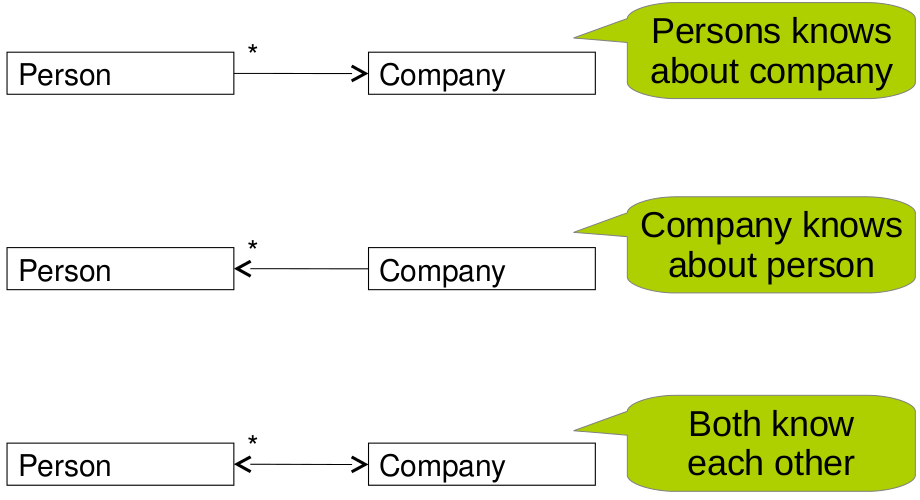
\includegraphics[width=0.5\textwidth]{img/association_directed.png}
	
	\item Aggregations
	\enumstart
		\item Variant of association
		\item Expresses a hierarchical part-of (has-a) relationship
		\item Classes can be part of several aggregates
	\enumend
	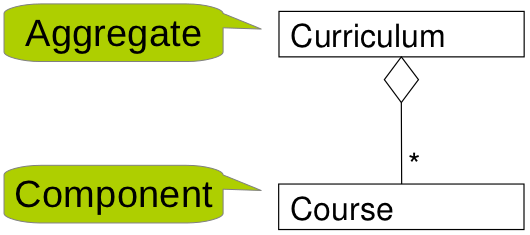
\includegraphics[width=0.5\textwidth]{img/aggregation.png}

	\item Composition
	\enumstart
		\item Expresses a strong aggregation
		\item No sharing of components
	\enumend
	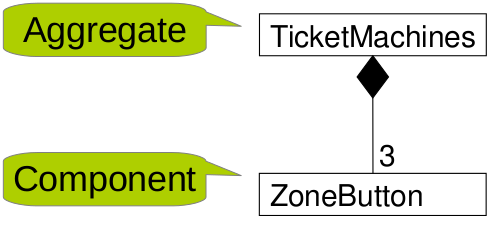
\includegraphics[width=0.5\textwidth]{img/composition.png}
	
	\item Generalization
	\enumstart
		\item Expresses a kind-of (is-a) relationship
		\item Implemented by inheritance
		\item Simplifies model by eliminating redundancy
	\enumend
	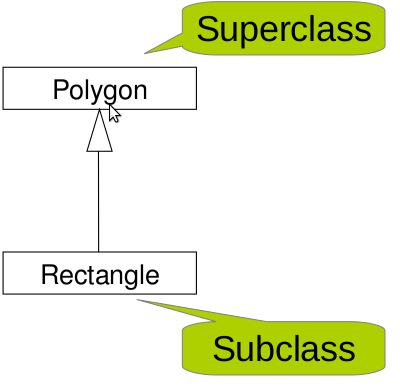
\includegraphics[width=0.5\textwidth]{img/generalization.png}
	
	\item Dependency
	\enumstart
		\item Express that changes to class B may cause changes to class A
		\enumstart
			\item A calls methods of B
			\item A mentions B as a parameter of a method
		\enumend
		\item Weaker then association, does not imply an attribute
	\enumend
	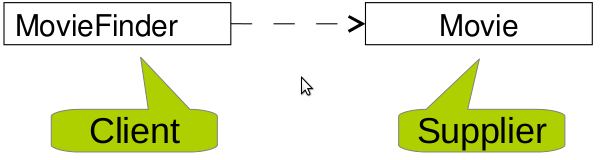
\includegraphics[width=0.5\textwidth]{img/dependency.png}
\enumend

\subsubsection{Object diagram}
\enumstart
	\item Shows snapshots of objects at a point in time
	\\ 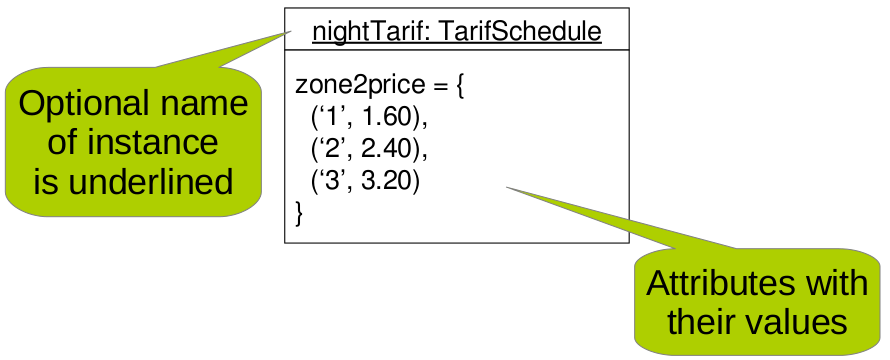
\includegraphics[width=0.5\textwidth]{img/object_diagram.png}
\enumend

\subsubsection{Identifying classes}
\enumstart
	\item Application domain approach
	\enumstart
		\item Ask application domain expert to identify relevant abstractions
	\enumend

	\item Syntactic approach
	\enumstart
		\item Extract participating objects from flow of events in problem statement
		\item Use noun-verb analysis to identify classes
		\enumstart
			\item Nouns: candidates for classes
			\item Verbs: candidates for operations
			\item Works well for short, structured text
		\enumend
	\enumend

	\item Design patterns approach
	\enumstart
		\item Use reusable design patterns
	\enumend

	\item Component-based approach
	\enumstart
		\item Identify existing solution classes
	\enumend

	\item Different kinds of objects
	\enumstart
		\item Entity objects
		\enumstart
			\item Represent the persistent information tracked by the system
			\item Application domain objects
			\item Changes rarely
		\enumend
		\item Boundary objects
		\enumstart
			\item Represent the interaction between the user and the system
			\item Changes very often
		\enumend
		\item Control objects
		\enumstart
			\item Represent the control tasks performed by the system
			\item Usually no concrete counterpart in the real world
			\item Changes often
		\enumend
	\enumend
	\item Stereotypes
	\enumstart
		\item Identifies the different kinds of objects in UML
		\\ 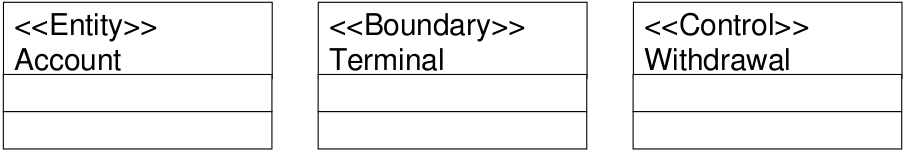
\includegraphics[width=0.5\textwidth]{img/stereotypes.png}
	\enumend
\enumend

\subsubsection{Mapping classes to code}
\enumstart
	\item Generalization
	\enumstart
		\item Inheritance
		\item Interfaces
	\enumend

	\item Visibility
	\enumstart
		\item Save connected objects as attributes
	\enumend

	\item Qualified association
	\enumstart
		\item Save a name for every connected object
		\item Probably use a dictionary datastructure
	\enumend

	\item Multiplicities
	\enumstart
		\item Ensure them by invariants
	\enumend
\enumend

\subsubsection{Sequence diagrams}
\enumstart
	\item Descripes operations of the class model
	\\ 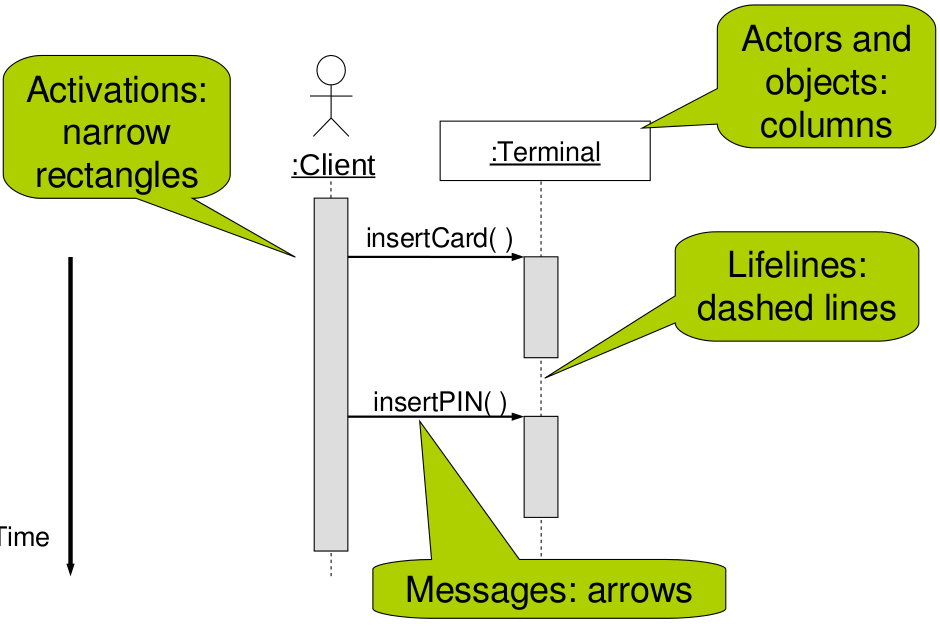
\includegraphics[width=0.5\textwidth]{img/sequence_diagram.png}

	\item Nested messages
	\\ 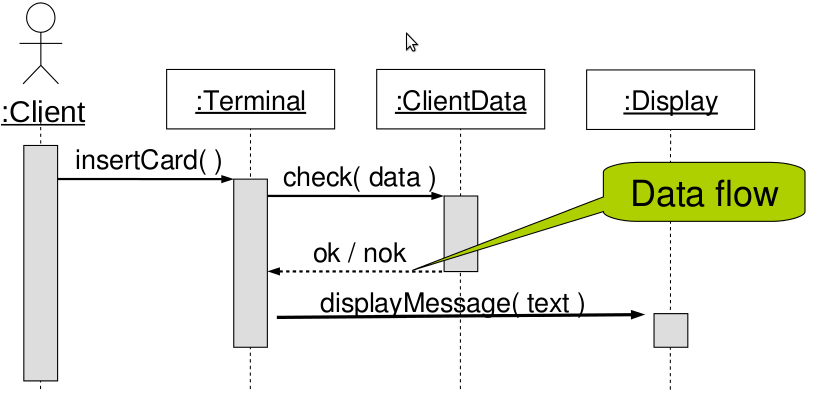
\includegraphics[width=0.5\textwidth]{img/nested_messages.png}
	
	\item Creation and destruction
	\\ 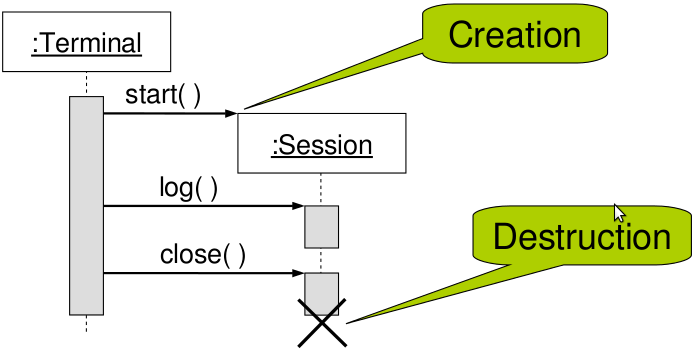
\includegraphics[width=0.5\textwidth]{img/creation_destruction.png}
	
	\item Recommended layout
	\\ 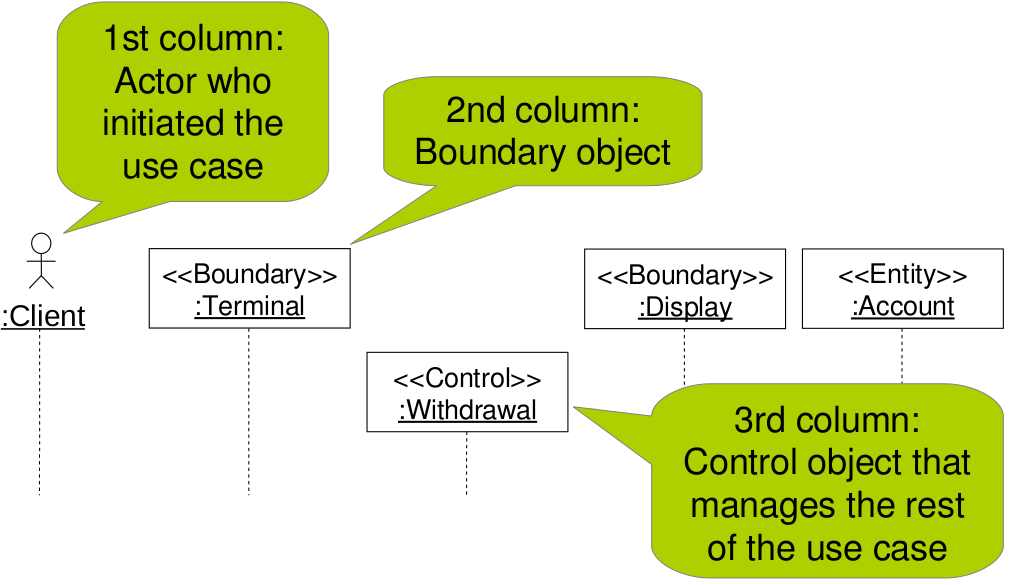
\includegraphics[width=0.5\textwidth]{img/recommended_layout.png}
	
	\item Heuristics for sequence diagrams
	\enumstart
		\item Creation of objects
		\enumstart
			\item Control objects are created at the initiation of the usecase
		\enumend
		\item Access of objects
		\enumstart
			\item Entity objects are accessed by control and boundary objects
			\item Entity objects never access control or boundary objects
		\enumend
	\enumend

	\item Structures
	\enumstart
		\item Fork structure
		\enumstart
			\item Dynamic behaviour concentrated in a single object
			\item Usually a control object
			\item Operations can change order
			\\ 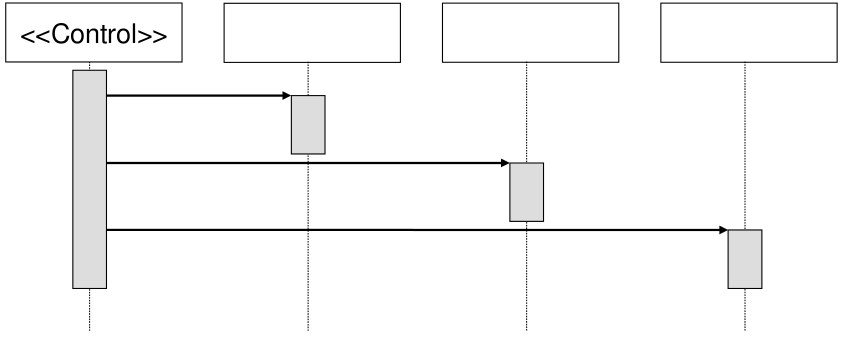
\includegraphics[width=0.5\textwidth]{img/fork_structure.png}
		\enumend
		\item Stair structure
		\enumstart
			\item Dynamic behaviour is distributed
			\item Objects delegate responsibility
			\item Chose when operations will always be performed in the same order
			\\ 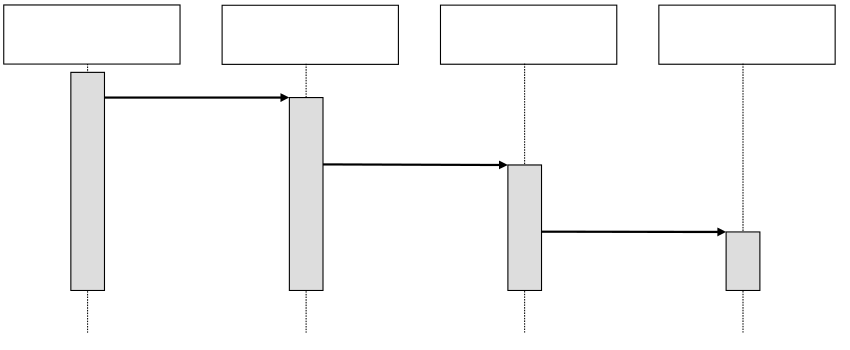
\includegraphics[width=0.5\textwidth]{img/stair_structure.png}
		\enumend
	\enumend
\enumend

\subsubsection{State machine diagrams}
\enumstart
	\item Long-living objects often have state-dependant behavior
	\enumstart
		\item Typical for control objects
		\item Sometimes also for entity objects
		\item Never for boundary objects
	\enumend
	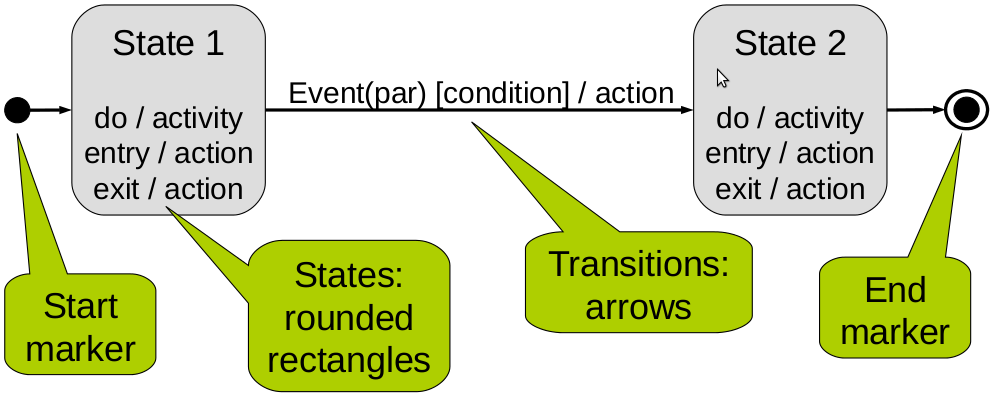
\includegraphics[width=0.5\textwidth]{img/state_diagram.png}
	\item Event: Something that happens at a point in time
	\item Action: Operation in response to an event
	\item Activity: Operation performed as long as operation is in some state
	\item Events can have different effects depending on guard conditions
	\\ 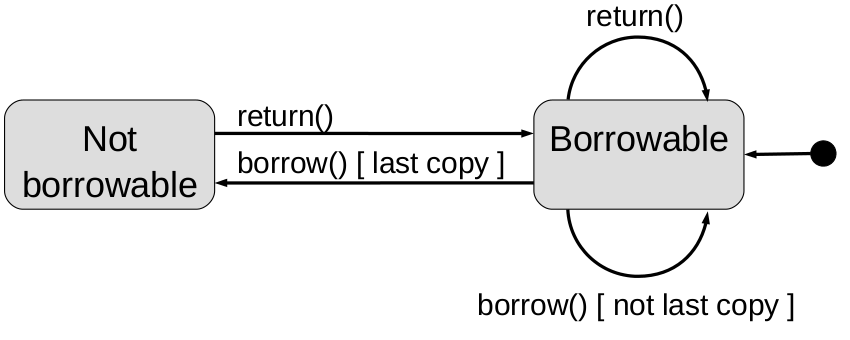
\includegraphics[width=0.5\textwidth]{img/guard_condition.png}
	\item Some state diagrams do not have end markers
	\item State diagrams can be nested (a state has its own state diagram)
\enumend

\subsubsection{Model-driven development}
\enumstart
	\item Idea: Work on the level of design models
	\item Generate code automatically (forward engineering)
	\item Advantages
	\enumstart
		\item Supports different implementation platforms
		\item Frees programmers from recurring activities
		\item Leads to uniform code
	\enumend
	\item Problems
	\enumstart
		\item Models may use different abstractions than programming language
		\item Models are incomplete specifications
		\item Models are informal
		\item Modification of generated code complicates things
	\enumend
	\item Reality
	\enumstart
		\item Mode-driven development is only a buzzword
		\item Code generation works only for very basic code
	\enumend
\enumend

\section{Design patterns}
\enumstart
	\item Motivation
	\enumstart
		\item Designing object-oriented software isn't trivial
		\enumstart
			\item Create classes at the right granularity
			\item Establish inheritance hierarchies
			\item Establish relationships between classes
			\item Define interfaces
		\enumend
		\item Good design
		\enumstart
			\item Solves the current problem
			\item Is general enough for future requirements
		\enumend
		\item You're not the first one to write software
		\item Goal: Reuse solutions that worked in the past
		\item Design patterns: Reusable solution to a commonly occuring problem in software design
	\enumend
\enumend

\subsection{Composite pattern}
\enumstart
	\item A program manipulates
	\enumstart
		\item individual objects
		\item Compositions of objects that form a part-whole hierarchy
	\enumend
	\item Want to allow algorithms to treat individual objects and compositions of objects uniformly
	\\ 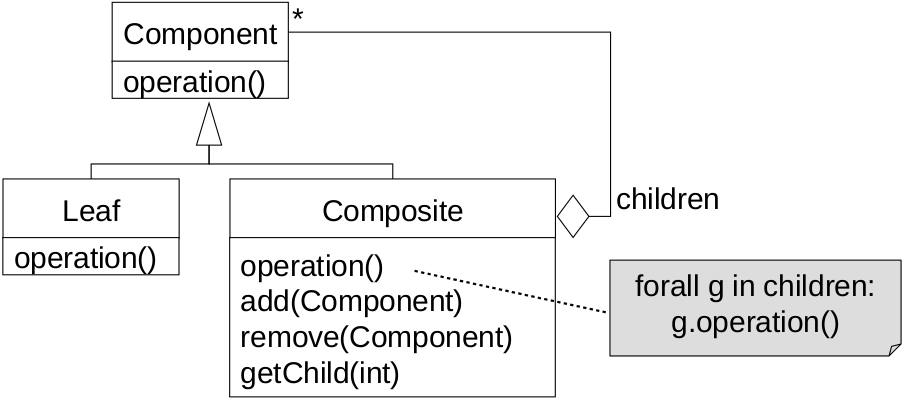
\includegraphics[width=0.5\textwidth]{img/composite_pattern.png}
	\item Properties
	\enumstart
		\item Makes clients simple: Composite objects used like primitive objects
		\item Easy to add new kinds of objects
		\item Can make the design too general
	\enumend
	\item Implementation
	\enumstart
		\item Explicit parent references
		\item Sharing components - reduces memory requirements (flyweight-pattern)
		\item Order of children
		\item Caching to improve performance
		\item Data structure for storing components
	\enumend
\enumend

\subsection{Object adapter pattern}
\enumstart
	\item Problem: incompatible interfaces
	\\ 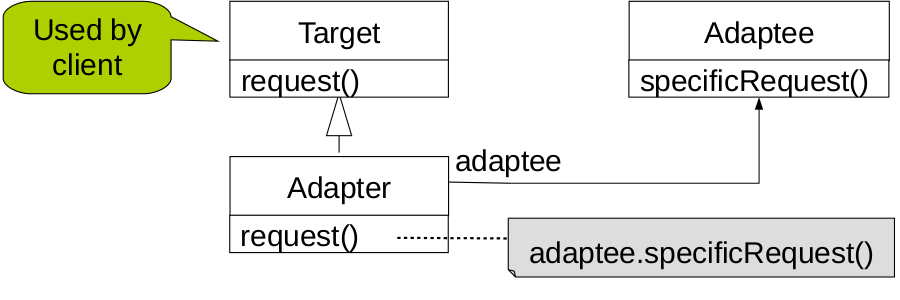
\includegraphics[width=0.5\textwidth]{img/object_adapter_pattern.png}
	\item Structure
	\enumstart
		\item Adapter forwards to adaptee
		\item Subtyping used to specify interface to adapter
		\item Target and adaptee exist before adapter
		\item Target may be an interface in Java
	\enumend
	\item Properties
	\enumstart
		\item Can adapt multiple existing subclasses without subclassing each of them
		 \item Ovelleo.orgrride adaptee's behaviour is harder, because of object schizophrenia
	\enumend
\enumend

\subsubsection{Object schizophrenia}
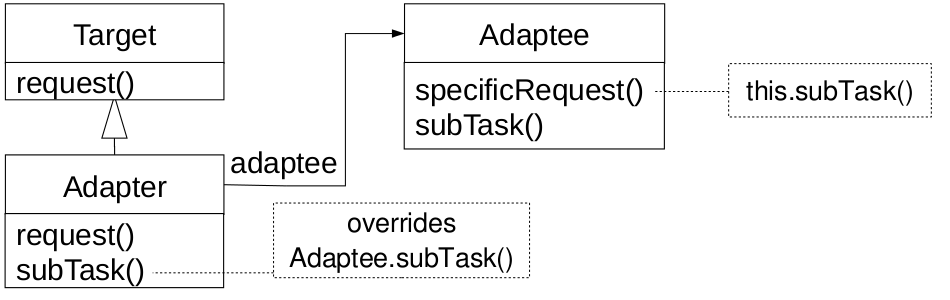
\includegraphics[width=0.5\textwidth]{img/object_schizophrenia.png}
\enumstart
	\item Forwarding request() to specificRequest() will not lead to a call to Adapter.subTask()
	\item Problem: Two objects represent one conceptual object
\enumend

\subsection{Class adapter pattern}
\enumstart
	\item Alternative to object adapter
	\\ 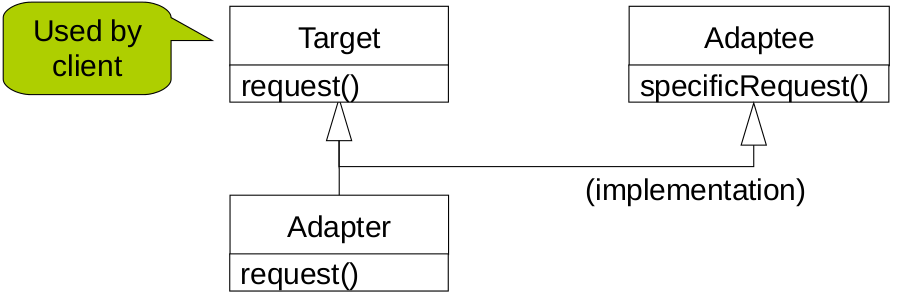
\includegraphics[width=0.5\textwidth]{img/class_adapter_pattern.png}
	\item Structure
	\enumstart
		\item Adapter inherits implementation from adaptee
		\item Target and adaptee exist before adapter
		\item Target must be an interface in Java
	\enumend
	\item Properties
	\enumstart
		\item Adapts one class at a time
		\item Can override some of adaptees behaviour
		\item Only one object, no indirection
	\enumend
\enumend

\subsection{Abstract factory pattern}
\enumstart
	\item Problem: create objects without knowing their concrete class
	\\ 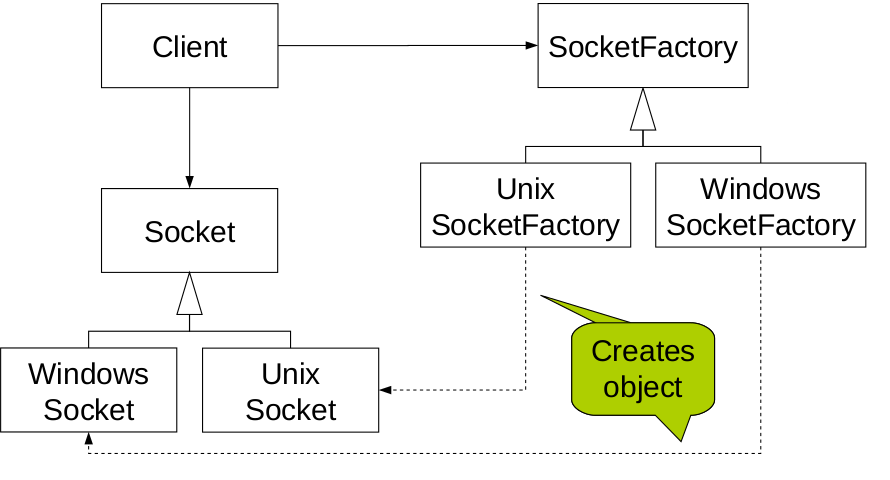
\includegraphics[width=0.5\textwidth]{img/abstract_factory_pattern.png}
	\item Applicability
	\enumstart
		\item System should be independant of how its classes are created, composed and represented
		\item Multiple families of related classes - Must decide on one family
		\item Provide a library of classes and reveal only their interfaces, not their implementations
	\enumend
	\item Properties
	\enumstart
		\item Isolates concrete classes
		\enumstart
			\item Helps control what classes are instantiated
			\item Isolates classes from implementation classes
		\enumend
		\item Exchanging product families is easy
		\enumstart
			\item Concrete factory appears only once in a program
		\enumend
		\item Supporting new kinds of products is difficult
		\enumstart
			\item Affects interface of abstract factory and all concrete factories
		\enumend
	\enumend
\enumend

\subsection{Singleton pattern}
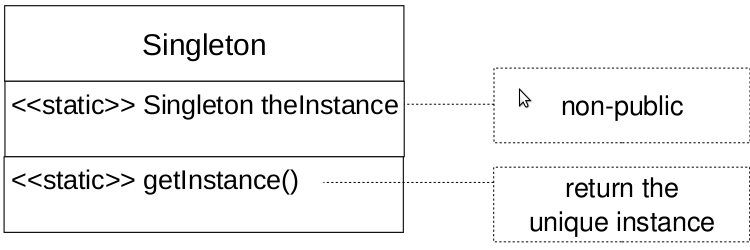
\includegraphics[width=0.5\textwidth]{img/singleton_pattern.png}
\enumstart
	\item Exactly one instance of a class
	\item Generalizable to any number of instances
	\item Sometimes part of the programming-language
	\item Applicability
	\enumstart
		\item Ensure that a class has only one instance and provide a global point of access to it
		\item A global variable alone is insufficient - May still have multiple instances
	\enumend
\enumend

\subsection{Iterator pattern}
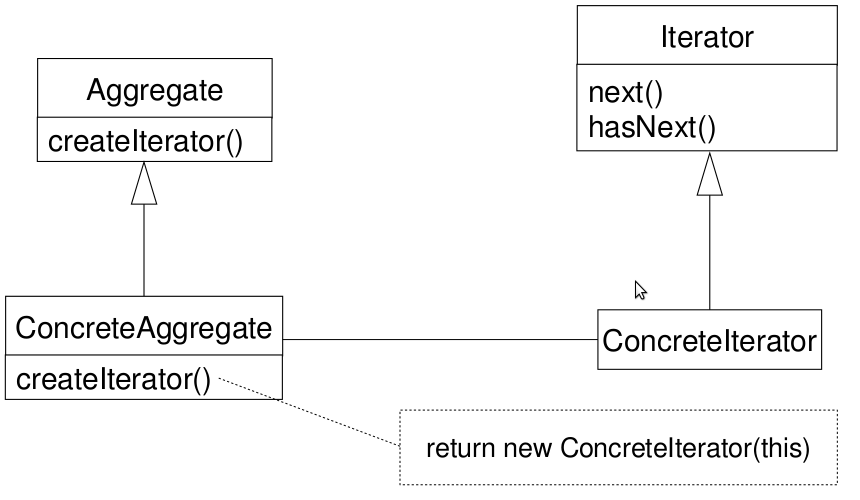
\includegraphics[width=0.5\textwidth]{img/iterator_pattern.png}
\enumstart
	\item Applicability
	\enumstart
		\item Provides a way to access the elements of a container without exposing it's internals
		\item Support multiple traversals of aggregate objects
		\item Provide a uniform interface for traversing different kinds of aggregate structures
	\enumend
	\item Properties
	\enumstart
		\item Separate implementation of traversals from implementation of aggregate object
		\item Simplifies the aggregates interface - Can support different kinds of traversals with a single method iterator()
		\item Easy to switch between variations of traversal
	\enumend
\enumend

\subsection{Observer pattern}
\enumstart
	\item Problem: Maintain Consistency between loosely coupled objects
	\\ 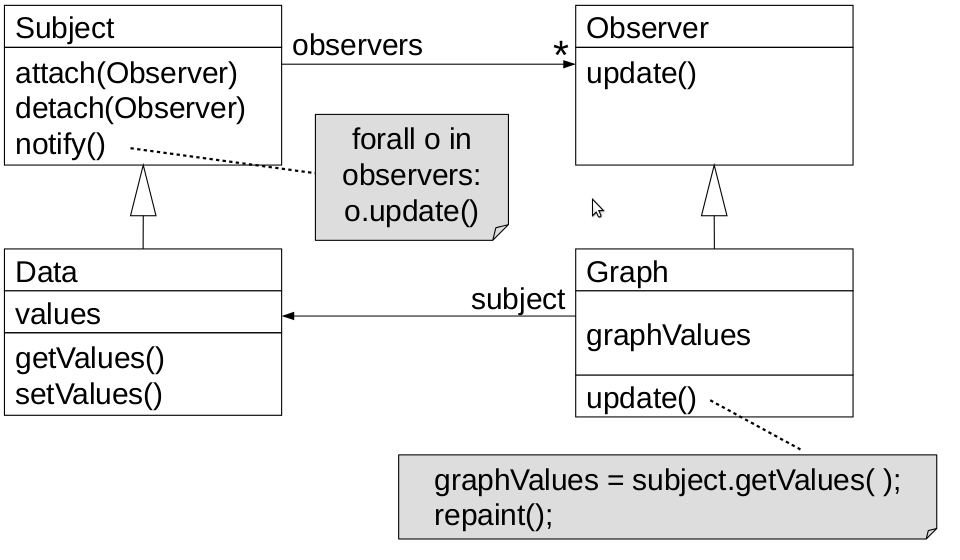
\includegraphics[width=0.5\textwidth]{img/observer_pattern.png}
	\item Applicability
	\enumstart
		\item Many dependant objects must be informed, when one object (subject) changes its state
		\item Subject should not depend on its dependants
	\enumend
	\item Properties
	\enumstart
		\item Loose coupling - alows layering
		\item Support for broadcast communication - add/remove observers dynamically
		\item Also known as: Listener, Publish-Subscribe
	\enumend
\enumend

\subsection{Strategy pattern}
\enumstart
	\item Problem: Exchangeable algorithms
	\\ 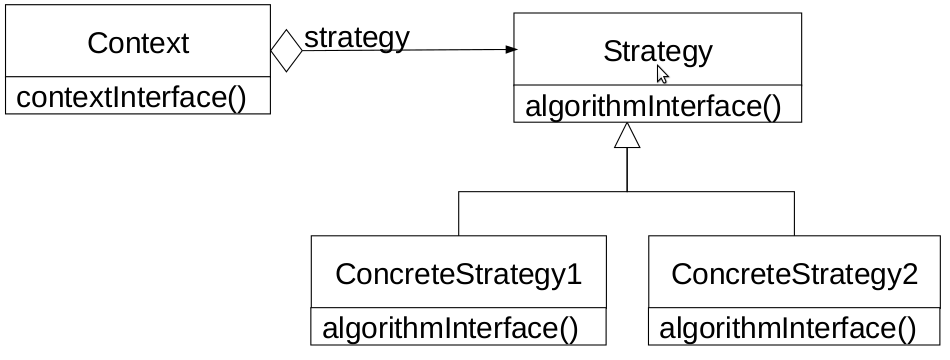
\includegraphics[width=0.5\textwidth]{img/strategy_pattern.png}
	\item Applicability
	\enumstart
		\item An algorithm has different variations, each appropriate for a different situation
		\item Want to vary the algorithm without changing the client
		\item Algorithms are complex and should be encapsulated in their own classes
	\enumend
	\item Properties
	\enumstart
		\item Supports families of algorithms
		\item Alternative to inheritance
		\enumstart
			\item Behaviour not hardwired but dynamically exchangeable
			\item Seperates context from algorithm - easier to maintain
		\enumend
		\item Communication overhead - Must pass all required data to algorithm
	\enumend
\enumend

\subsection{Template method pattern}
\enumstart
	\item Problem: Refinement of algorithms
	\\ 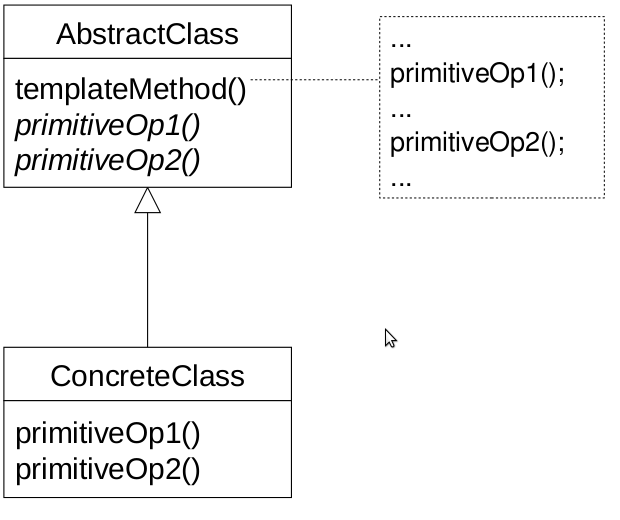
\includegraphics[width=0.5\textwidth]{img/template_method_pattern.png}
	\item Applicability
	\enumstart
		\item Want to refine steps of an algorithm without changing its overall structure
		\item An algorithm has several variant and an invariant part
		\item Want to avoid code duplication of the invariant part
	\enumend
	\item Properties
	\enumstart
		\item Inverted call-structure - Parent calls child, not the other way around
		\item Abstract class may define defaults for some primitive operations
		\item Primitive operations are often non-public
	\enumend
\enumend

\subsection{Visitor pattern}
\enumstart
	\item Problem: Operate on an object structure
	\\ 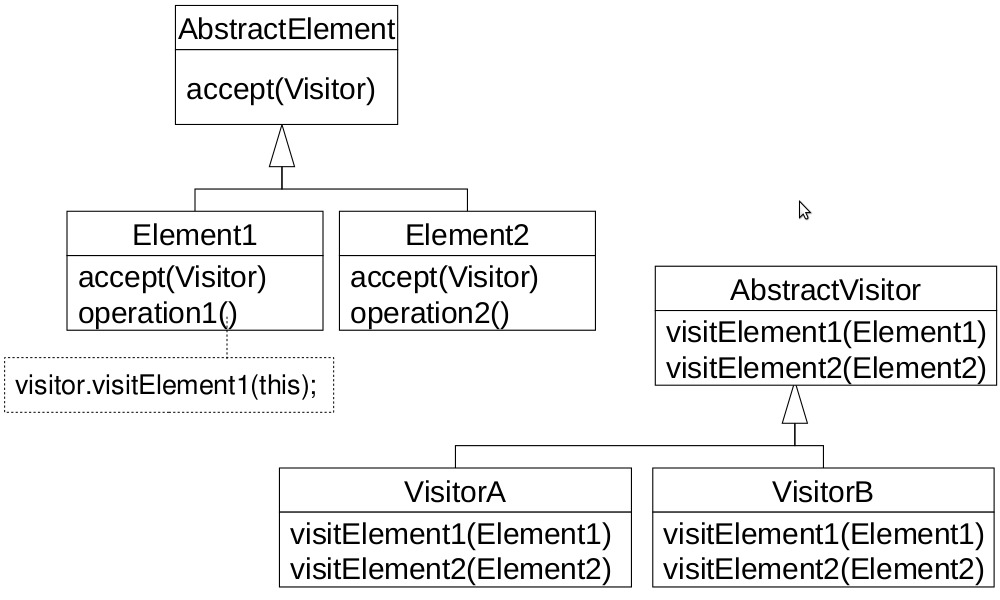
\includegraphics[width=0.5\textwidth]{img/visitor_pattern.png}
	\item Applicability
	\enumstart
		\item Object structure with many classes
		\item Many operations to be performed
		\item Operations depend on concrete class of object
		\item Classes of object structure rarely change
	\enumend
	\item Properties
	\enumstart
		\item Changing/adding operations is easy - each operations encapsulated in one class
		\item Changing the object structure is difficult - must adapt all visitors
		\item implements double dispatch in a language with single dispatch
	\enumend
\enumend

\subsubsection{Double dispatch}
\enumstart
	\item Objects have a static and a dynamic type
	\item Dynamic dispatch - choose method based on dynamic types
	\item Often: Single dispatch on method receiver
	\item Sometimes needed: Double dispatch on receiver and arguments
\enumend

\subsection{Facade pattern}
\enumstart
	\item Problem: Unified interface for a subsystem
	\\ 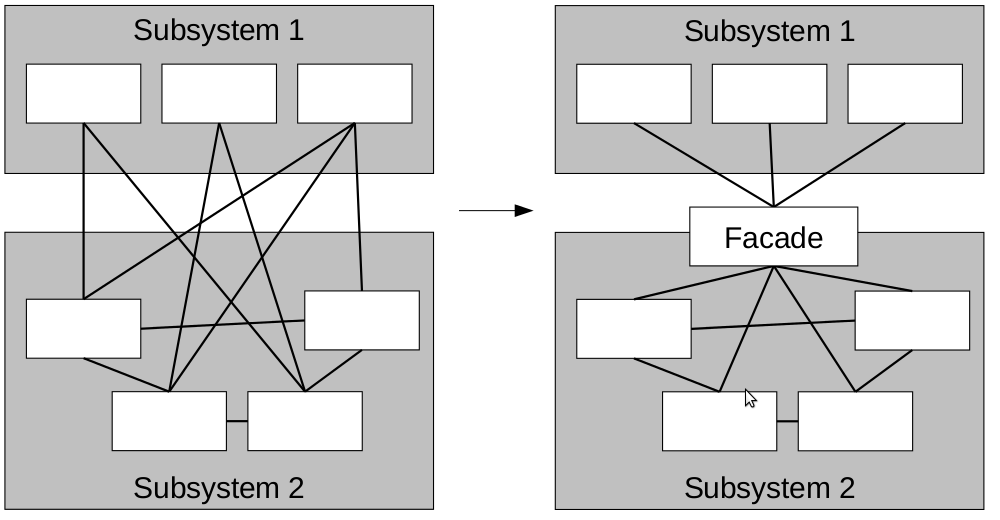
\includegraphics[width=0.5\textwidth]{img/facade_pattern.png}
	\item Properties
	\enumstart
		\item Highlevel interface that makes subsystem easier to use
		\item Reduces coupling
		\item Most of the time, facade need not to be changed when subsystem changes
		\item Does not prevent direct usage of objects within a subsystem
	\enumend
\enumend

\subsection{Command pattern}
\enumstart
	\item Problem: Encapsulate actions
	\\ 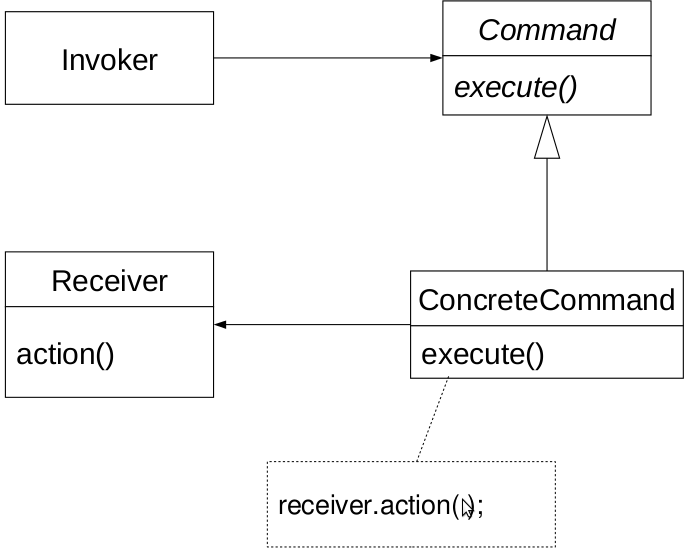
\includegraphics[width=0.5\textwidth]{img/command_pattern.png}
	\item Applicability
	\enumstart
		\item Actions to be performed should be first class entities
		\item Specify, queue, and execute requests at different times
		\item Support undo/redo
	\enumend
	\item Properties
	\enumstart
		\item Decouples the object that invokes an operation from the one that knows how to perform it
		\item Commands can be extended and manipulated like any other object
		\item Can assemble commands into macro commands
		\item Adding new commands is easy - no need to change other classes
	\enumend
\enumend

\subsection{Bridge pattern}
\enumstart
	\item Problem: Vary abstraction and implementation independantly
	\\ 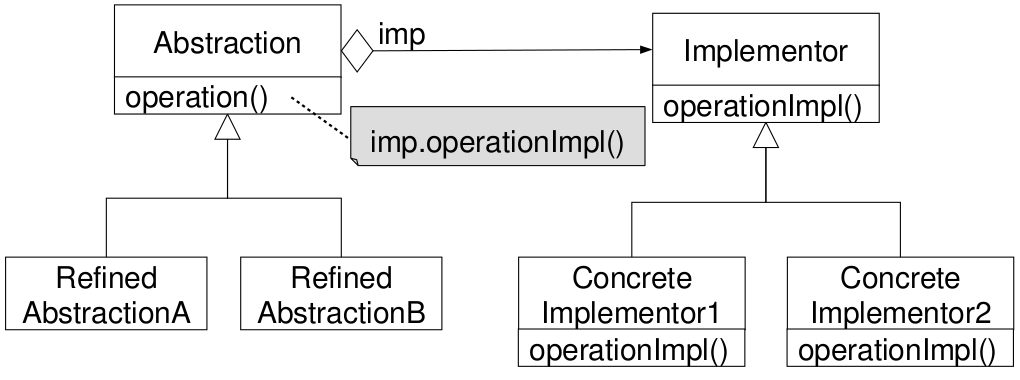
\includegraphics[width=0.5\textwidth]{img/bridge_pattern.png}
	\item Applicability
	\enumstart
		\item Have two dimensions that vary independantly
		\item Want to avoid explosion of class hierarchy
		\item Changes in implementation should not affect clients
	\enumend
	\item Properties
	\enumstart
		\item Implementations of an interface can be exchanged dynamically
		\item Can extend abstraction and implementation hierarchy independantly
		\item Hides implementation details from client
	\enumend
	\item Bridge vs. Adapter
	\enumstart
		\item Both used to hide details of underlying implementation
		\item Adapter
		\enumstart
			\item Makes unrelated components work together
			\item Applied after a system is designed
		\enumend
		\item Bridge
		\enumstart
			\item Used up-front to design an extensible system
		\enumend
	\enumend
\enumend

\section{Coding practice}

\subsection{Naming conventions}
\enumstart
	\item Goal: Consistency
	\item Consistency within an environment improves code readability
	\\ 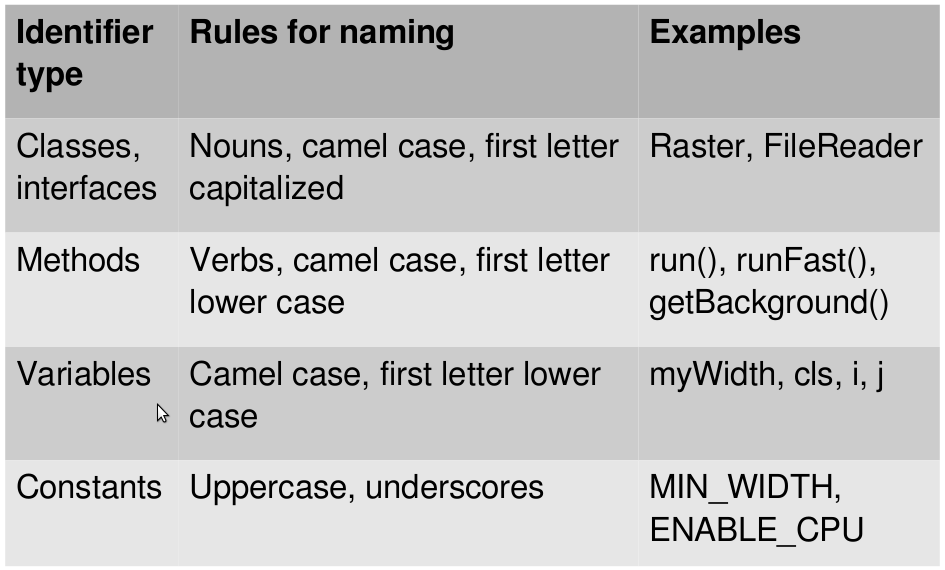
\includegraphics[width=0.5\textwidth]{img/java_naming_conventions.png}
	\item Method names
	\enumstart
		\item Goal: Help understand what a method does without inspecting its implementation
		\item Setters and getters of fields: getBlub(), setBla()
		\item Status methods: isFoo(), hasBar()
		\item Names that suggest side-effect freedom: findX()
		\item Names that suggest to have side-effects: openConnection()
	\enumend
	\item Longer names $\rightarrow$ better comprehension of source code
	\item But names can also be too long
\enumend

\subsection{Code Formatting}
\enumstart
	\item Consistent indentation
	\item Use spaces consistently
	\item Use brackets consistently
\enumend

\subsection{Documentation}
\enumstart
	\item API documentation
	\enumstart
		\item Help others to use your code without understanding its details
		\item Javadoc
	\enumend
	\item Code documentation
	\enumstart
		\item Ideally, the code makes clear what it does
		\item Comments should explain why you do it
	\enumend
\enumend

\subsection{Software clones}
\enumstart
	\item Copy-and-paste of source code fragments
	\item Take a working piece of code and reuse it by adapting it slightly
	\item Problem:
	\enumstart
		\item The same bug might occur multiple times
		\item Lines of code to maintain increase without adding new functionality
		\item When changing one clone, must change all clones, but cloning is not documented
	\enumend
	\item Solution:
	\enumstart
		\item Encapsulate reusable code into methods
		\item Replace clones by call to the reusable method
		\item Whenever you use copy-and-paste, think about other reuse mechanisms
	\enumend
\enumend

\subsection{Liskov's substitutability principle}
\enumstart
	\item A subclass instance used through the superclass type should behave like a superclass instance
	\item Bad Practice: Subclasses that reuse the superclass implementation but that do not semantically substitute the superclass
\enumend

\subsection{Test-driven development}
\enumstart
	\item Assumption that testing is a fundamental part of development
	\item Philosophy: Testing drives development
	\enumstart
		\item Testing doesn't occur after implementing
		\item Testing occurs before and during the implementation
	\enumend
	\item Result: increased confidence when changing code
	\item Steps
	\enumstart
		\item Add a test
		\item Run all tests and see the new one fail
		\item Change production code
		\item Run all tests and see them pass
	\enumend
	\item Philosophy: Production code is written to make failing tests pass
	\item How to test one class if other classes are still missing?
	\enumstart
		\item Create mock objects that simulate the behaviour of missing classes
		\item Same interface as real objects
		\item Simpler implementation (e.g. return default values)
		\item Also usefull if other classes exist but are difficult to integrate into a unit test
	\enumend
	\item How many tests do we need?
	\enumstart
		\item Testing cannot prove your program correct
		\item Should cover all functionality of the class under test
		\item Code coverage quantifies which percentage of your code is exercised by tests
	\enumend
\enumend

\subsection{Version-control}
\enumstart
	\item All software has different versions
	\enumstart
		\item Each time a developer changes the code
		\item Versions within the development cicle
		\item Versions for different platforms
	\enumend
	\item Why use version-control?
	\enumstart
		\item Allow more than one developer to work on the code
		\item Recreate old versions
		\item Change log
		\item Find who is responsible for a piece of code
	\enumend
\enumend

\section{Refactoring}
\enumstart
	\item Many programs are designed or implemented in a suboptimal way
	\enumstart
		\item Poor performance
		\item Hard to maintain
		\item Hard to extend
	\enumend
	\item Definition: Behaviour-preserving changes that improve the internal structure of existing code
	\item Why to refactor?
	\enumstart
		\item improves the design of the software
		\item makes code easier to understand
		\item helps to find bugs
		\item helps to program faster
	\enumend
	\item When to refactor?
	\enumstart
		\item When adding a new feature
		\item When fixing a bug
		\item When doing code review
	\enumend
	\item What to refactor?
	\enumstart
		\item Duplicate code
		\item Long methods
		\item Large classes
		\item Long or recurring switch statements
		\item changes that imply many other changes
	\enumend
	\item Discussion
	\enumstart
		\item Refactoring vs performance
		\enumstart
			\item Refactoring may cause slowdown
			\item But: for well-defined code, its much easier to tune performance
		\enumend
		\item Refactoring vs management
		\enumstart
			\item Effects of bad design show up after some time
			\item Refactoring enables long-term evolution
		\enumend
		\item Sometimes rewriting is easier than refactoring
	\enumend
\enumend

\subsection{Composing methods}
\enumstart
	\item Adapt the way code is packaged into methods
	\item Break large methods into smaller ones
	\item Combine small methods into a larger one
	\item Goal: Methods that are small enough to be understood easily
\enumend

\subsubsection{Extract method}
\enumstart
	\item Steps
	\enumstart
		\item Turn code fragment into a method whose name explains the purpose of the method
		\item Turn local variables used in the fragment into parameters of the method
		\item Turn local variables defined in the code fragment into the methods return value
	\enumend
	\item Benefits
	\enumstart
		\item Reuse: finer-graned methods are more likely to be reused
		\item Adaptability: Overriding the extracted code becomes easier
		\item Clarity: The higher-level method becomes easier to read
	\enumend
\enumend

\subsubsection{Inline methods}
\enumstart
	\item Given: A methods body is just as clear as its name
	\item Steps
	\enumstart
		\item Put the methods body into the body of the callers and remove the method
	\enumend
	\item Opposite of Extract method
	\item Apply only if method is not polymorphic
	\item Benefits
	\enumstart
		\item Clarity: Avoid useless indirection
		\item Enables other refactorings
	\enumend
\enumend

\subsubsection{Replace method with method object}
\enumstart
	\item Given: Large method that is difficult to decompose because of local variables
	\item Steps
	\enumstart
		\item Create a new class with a field for each local variable and each parameter of the method, and for the object that hosts the method
		\item Add constructor that initializes all fields
		\item Copy the original methods code into a new method compute()
		\item Replace the method with code that instantiates the new class and calls compute()
	\enumend
	\item Benefits
	\enumstart
		\item Enables other refactorings
		\item Can decompose a method, even if it uses many local variables
	\enumend
\enumend

\subsection{Moving features between objects}
\enumstart
	\item Where to put which responsibilities?
	\item Goal: improve assignments of fields and methods to classes
\enumend

\subsubsection{Move method}
\enumstart
	\item Given: A method using (or used by) more features of another class then its current class
	\item Steps
	\enumstart
		\item Check that superclasses and subclasses do not declare the method
		\item Move the method to the target class and adjust it - pass fields of source object or the source object itself
		\item Turn source method into a delegating method or remove it altogether
	\enumend
	\item Benefits
	\enumstart
		\item Reduce coupling of classes
		\item Shrink a large class by reducing its responsibilities
		\item Most usefull with other moves of fields and methods
	\enumend
\enumend

\subsubsection{Move field}
\enumstart
	\item Similar to "move method"
	\item Applicable if field is used by another class more than by its own class
	\item Create a new field in the target class and change all its users
\enumend

\subsubsection{Extract class}
\enumstart
	\item Given: A class does work that should be done by two
	\item Steps
	\enumstart
		\item Create a new class and reference it from the old class
		\item Use "move field" on each field
		\item Use "move method" on each method - start with lower level methods
	\enumend
	\item Benefits
	\enumstart
		\item Increased encapsulation
		\item Counteracts the tendency to add more and more features to classes
	\enumend
\enumend

\subsubsection{Inline class}
\enumstart
	\item Counterpart of "extract class"
	\item Apply if a class has few or no responsibilities
	\item Move all features into the other class and remove the old class
\enumend
	
\subsubsection{Hide delegate}
\enumstart
	\item Given: client calls a delegate class via a server object
	\item Steps
	\enumstart
		\item For each method of the delegate, create a delegating method on the server class
		\item Adjust the client to call the server
		\item Remove the servers method that returns the delegate (if not needed anymore)
	\enumend
	\item Benefits
	\enumstart
		\item Encapsulation - client becomes independent of how the server accesses the delegate
		\item Reduced coupling - delegate class is hidden from the client
	\enumend
\enumend

\subsubsection{Remove middle man}
\enumstart
	\item Counterpart of "hide delegate"
	\item If a class does too much delegation, let the client call the delegate directly
	\item Consequence: Avoids delegating methods, but reduces encapsulation
\enumend

\subsection{Organizing data}
\enumstart
	\item The best way to represent your data may change over time
	\item Goal: adapt data representation
\enumend

\subsubsection{Replace data with object}
\enumstart
	\item A data item that needs additional data or behaviour
	\item Steps
	\enumstart
		\item Create a class for the value, add a final field for the value
		\item Change the type of the field in the source class
		\item Let the getter in the source class call the getter of the new class
		\item Let the setter in the source class create a new instance of the new class
	\enumend
	\item Benefits
	\enumstart
		\item Enable adding fields and methods to the data item
		\item Deals with evolution, where a simple piece of data becomes more important over time
	\enumend
\enumend

\subsubsection{Replace array with object}
\enumstart
	\item Given: an array that stores data records
	\item Steps
	\enumstart
		\item Create a class and give it a public field for the array
		\item Change all users of the array to use the new class
		\item For each element of the array, replace direct array access with getters and setters
		\item Replace the array field with a field for each array element
	\enumend
	\item Benefits
	\enumstart
		\item Understandability
		\item Maintainability
		\item Encapsulation - Getters and setters may perform checks without influencing the client
		\item May add behaviour to the class later on
	\enumend
\enumend

\subsection{Simplifying conditional expressions}
\enumstart
	\item Conditional logic is tricky
	\item Goal: Simplify or remove conditional expressions
\enumend

\subsubsection{Decompose conditional}
\enumstart
	\item Given: a complicated conditional statement
	\item Steps
	\enumstart
		\item Extract condition into its own method
		\item Extract then-part and else-part into their own methods
	\enumend
	\item Benefit: Code becomes easier to unserstand and bugs become easier to find
\enumend

\subsubsection{Consolidate conditional expressions}
\enumstart
	\item Givem: sequence of conditional tests with the same result
	\item Steps
	\enumstart
		\item Check that all conditionals are side-effect free
		\item Replace sequence with a single conditional
		\item Consider extracting combined condition into a method
	\enumend
	\item Benefit: Code becomes easier to unserstand
\enumend

\subsubsection{Replace conditional with polymorphism}
\enumstart
	\item Given: conditional that chooses behaviour based on the type of an object
	\item Steps
	\enumstart
		\item Create a class hierarchy (simple subclasses or the strategy pattern)
		\item Use "move method" to bring the conditional to the top of the hierarchy
		\item For each subclass, move the code from the conditional into a method that overrides the superclass method
	\enumend
	\item Benefits
	\enumstart
		\item Particularly usefull if the same conditional appears in many places
		\item Adding a new type becomes easier because only one location must be changed
		\item Avoid reimplementing dynamic dispatch which is already part of the language
	\enumend
\enumend

\subsection{Making method calls simpler}
\enumstart
	\item API design is important
	\item Goal: make using an api easier
\enumend

\subsubsection{Replace parameters with explicit methods}
\enumstart
	\item Given: method runs different code depending on the value of an enumerated parameter
	\item Steps
	\enumstart
		\item Create a method for each value of the parameter
		\item For each case of the conditional, call the appropriate method
		\item Change all callers of the original method to use the new methods
		\item Remove the original method
	\enumend
	\item Benefits
	\enumstart
		\item Clarity - Can understand API from method names, without looking at parameters
		\item Safety - Compile-time checking instead of unsafe parameter that determines the behaviour
	\enumend
\enumend

\subsubsection{Introduce parameter object}
\enumstart
	\item Given: group of parameters that naturally go together
	\item Steps
	\enumstart
		\item Create a new, immutable class to represent the parameters
		\item Add a parameter of the new class to all methods with the group of parameters
		\item Adapt all callers by passing a new instance of the new class
		\item For each parameter, move the directly passed parameter into the constructor of the new class
	\enumend
	\item Benefits
	\enumstart
		\item Understandability - Reduces the length of the parameter list
		\item May add behaviour to the new class later on
	\enumend
\enumend

\subsection{Dealing with generalization}
\enumstart
	\item Several refactoring to refine the use of inheritance
	\item Moving features up/down the hierarchy
	\item Refining the hierarchy
\enumend

\section{Testing}
\enumstart
	\item Why does Software contain bugs?
	\enumstart
		\item Ability to predict the behaviour of complex software is limited
		\item We make mistakes
		\enumstart
			\item Unclear requirements, miscommunication
			\item Wrong assumptions
			\item Design errors
			\item Coding errors
		\enumend
	\enumend
	\item Increasing software reliability
	\enumstart
		\item Fault avoidance
		\enumstart
			\item Statically - without executing the program
			\item Developement methodologies
		\enumend
		\item Fault detection
		\enumstart
			\item Dynamically - executing the program
			\item Static code checkers
		\enumend
		\item Fault tolerance
		\enumstart
			\item Recover from faults at runtime
		\enumend
	\enumend
	\item Error
	\enumstart
		\item Deviation of the observed behaviour from the required behaviour
		\item Functional
		\item Non-functional
	\enumend
	\item Testing
	\enumstart
		\item Process of executing a program to find errors
		\item Testing can only show the presence of bugs, not their absence
	\enumend
	\item Test harness - Collection of software and test data to automate test execution
	\\ 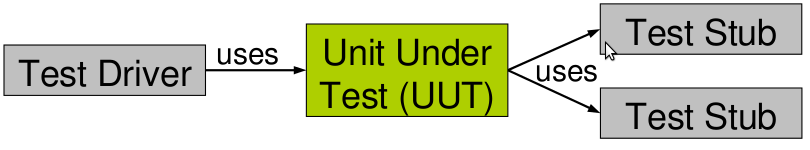
\includegraphics[width=0.5\textwidth]{img/test_harness.png}
	\enumstart
		\item Test driver - Applies test cases to UUT, including setup and cleanup
		\item Test stub - partial implementation that simulates the missing component by returning fake data
	\enumend
\enumend

\subsection{Unit testing}
\enumstart
	\item Testing of individual subsystems
	\item Goal: confirm that subsystem is correctly implemented and carries out the intended functionality
	\item To increase test coverage, test each method with several inputs
	\enumstart
		\item Cover valid and invalid inputs
		\item Cover different paths through the method
	\enumend
	\item Parameterized unit tests
	\enumstart
		\item Decouple test driver from test data
		\item Test data can be specified as values, ranges or random values
		\item Requires generic test oracles
	\enumend
	\item Rules
	\enumstart
		\item All tests should be fully automatic and check their own results
		\item Run tests frequently
		\item For each bug, write a unit test that exposes the bug
		\item Concentrate your tests on boundary conditions
		\item Test if exceptions are raised when things are expected to go wrong
		\item Better to write and run incomplete tests, than to not run tests at all
	\enumend
\enumend

\subsection{Integration testing}
\enumstart
	\item Testing of groups of subsystems
	\item Motivation: many faults result from the interaction of subsystems
	\item Goal: Test interfaces between subsystems
	\item Important: Unit test all classes in the subsystem before integration testing
	\item Strategies
	\enumstart
		\item Order in which the subsystems are selected for testing and integration
		\item Big-bang (non-incremental)
		\item Bottom-up
		\item Top-down
		\item Sandwich testing
		\item Continuous integration
	\enumend
\enumend

\subsection{System testing}
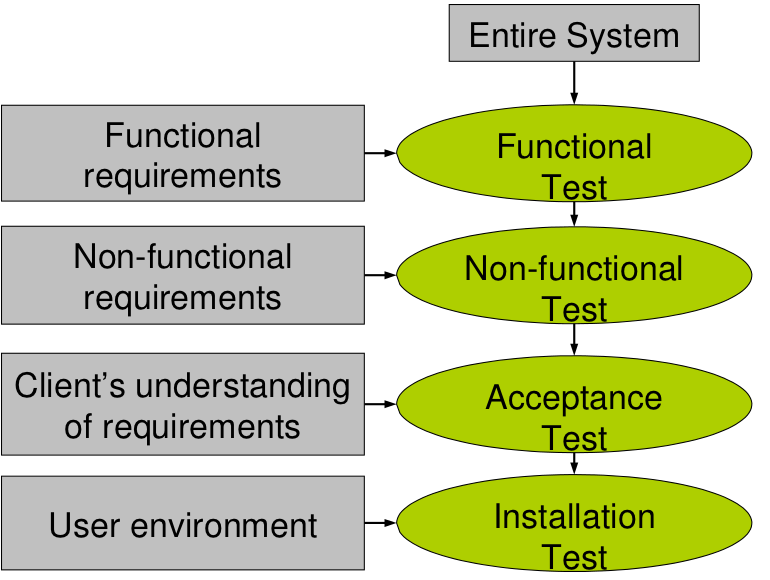
\includegraphics[width=0.5\textwidth]{img/system_testing.png}

\subsubsection{Functional testing}
\enumstart
	\item Testing functionality
	\item Treat system as a black box
	\item Test cases describe
	\enumstart
		\item Input data
		\item Flow of events
		\item Results to check
	\enumend
\enumend

\subsubsection{Non-functional testing}
\enumstart
	\item Stress testing (Explore limits of the system)
	\item Volume testing (Large amounts of data)
	\item Configuration testing (Various software and hardware configurations)
	\item Compatibility testing (e.g. backward compatibility)
	\item Security testing
	\item Timing testing
	\item Environmental testing (tolerance for heat, humidity, $\mathellipsis$)
	\item Recovery testing
	\item Usability testing
\enumend

\subsubsection{Acceptance testing}
\enumstart
	\item Demonstrate to customer
	\item Choice of test is made by clients
	\item Performed by the client
	\item Alpha-test / Beta-test
\enumend

\subsubsection{Installation testing}
\enumstart
	\item Test what users will do to install and set up the software
	\item Different environments
	\item Different configurations
\enumend

\subsubsection{Testing strategies}
\enumstart
	\item Exhaustive testing
	\item Random testing
	\item Functional-/black box testing
	\item Structural-/white box testing
\enumend

\subsection{Functional testing}
\enumstart
	\item Test suite should be complete w.r.t specification
	\item Test suite should be as precise as possible
	\item Treat the program as a black box
	\item Use functional specification as base for designing test cases
	\\ 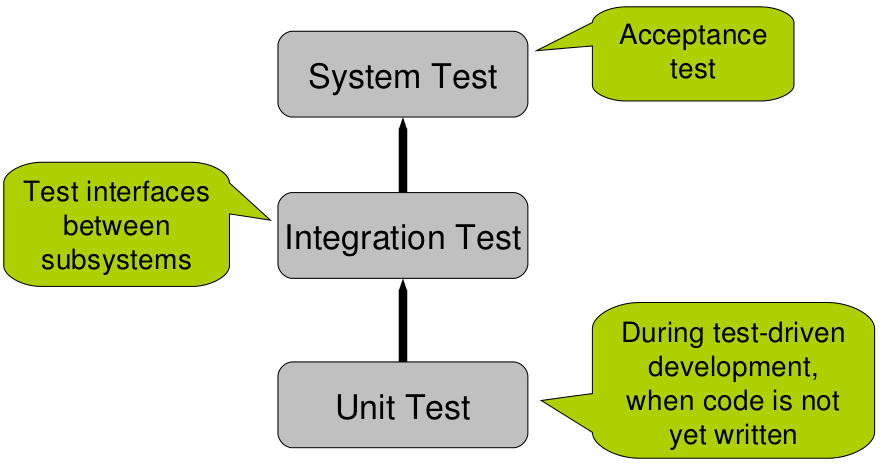
\includegraphics[width=0.5\textwidth]{img/functional_testing.png}
	\item Systematic functional testing
	\\ 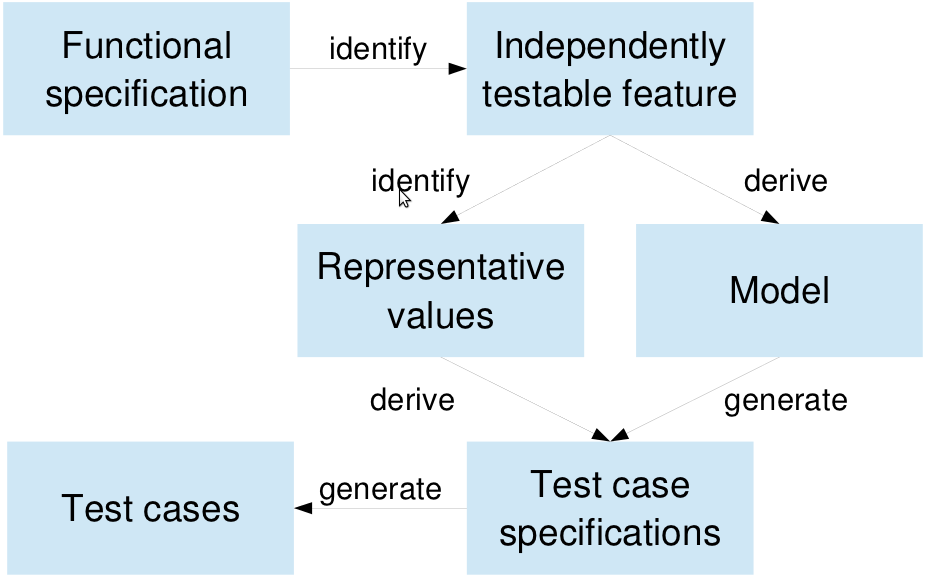
\includegraphics[width=0.5\textwidth]{img/systematic_functional_testing.png}
\enumend

\subsubsection{Functional specification}
\enumstart
	\item Describes technical requirement
	\item not how, but what it does
	\item informal or formal
\enumend

\subsubsection{Independently testable features}
\enumstart
	\item Decompose system into ITF
	\item ITF need not to correspond to classes or subsystems
\enumend

\subsubsection{Identifying representative values}
\enumstart
	\item Divide input into equivalence classes
	\item Chosing representatives for each equivalence class
	\enumstart
		\item Normal values
		\item Invalid values
		\item Special values (e.g. null, empty collection, $\mathellipsis$)
		\item Boundary values (Extreme values inside and outside of boundaries)
	\enumend
\enumend

\subsubsection{Test case specification}
\enumstart
	\item Combine representative values into test data
	\item Combinatorial testing (combine everything) $\rightarrow$ combinatorial explosion
	\enumstart
		\item Use semantic constraints to eliminate combinations
		\item Use domain knowledge to remove unnecessary combinations
	\enumend
	\item Pairwise testing
	\enumstart
		\item Bugs often depend on only a few variables
		\item Test only all pairs of input parameters
		\item Can generalize to $k$-way testing
		\item For $n$ parameters with $d$ values each, number of tests grows log in $n$ and quadratic in $d$
	\enumend
\enumend

\subsubsection{Model-based testing}
\enumstart
	\item Goal: derive test-cases from models
	\item Benefits:
	\enumstart
		\item Compare actual behaviour to modeled behaviour
		\item Measure coverage w.r.t model
		\item (Partly) automate test case generation
	\enumend
	\item Models
	\enumstart
		\item Structural model
		\enumstart
			\item Contains the main concepts manipulated by the system, their properties and relationships
			\item Relevant information
			\enumstart
				\item Classes and attributes
				\item Subtypes
				\item Associations and multiplicities
			\enumend
		\enumend
		\item Behavioral model
		\enumstart
			\item Sequence diagrams (usefull for integration testing)
			\item State diagrams (states $\rightarrow$ equivalence classes)
			\enumstart
				\item State coverage
				\item Transition coverage
			\enumend
		\enumend
		\item Decision structures
		\item Grammars
		\enumstart
			\item Complex inputs can often be described by a (contextfree) grammar
			\item Input of varying and unbounded size
			\item Input with recursive structure
			\item Test cases: Strings generated by the grammar
			\item Coverage criteria
			\enumstart
				\item Production coverage - each production must be used to create a t least one test case
				\item Boundary condition - generate for all productions: Min+1, Min, Max, Max-1
			\enumend
		\enumend
	\enumend
\enumend

\subsection{Structural testing}

\subsubsection{Control flow testing}
\enumstart
	\item Idea: Cover as many different flows of control as possible
	\item Control flow graph
	\enumstart
		\item Basic blocks as Nodes
		\item Flow of control as Edges
	\enumend
\enumend

\subsubsection{Basic Blocks}
\enumstart
	\item Sequence of statements with exactly one entry-point and one exit-point
	\item Whenever the first instruction is executed, the rest is executed once and in order
\enumend

\subsubsection{Intraprocedural control flow graph (CFG)}
\enumstart
	\item A CFG of a method is
	\enumstart
		\item A graph $(N, E)$
		\item $N$ contains the basic blocks of the method
		\item $E$ contains
		\enumstart
			\item edges $(a, b, c)$ where
			\enumstart
				\item the control flow goes from $a$ to $b$
				\item under the condition that $c$ holds
			\enumend
			\item an entry $(entry, a, true)$ to the first basic block
			\item edges $(b, exit, true)$ for each $b$ that ends with a return statement
		\enumend
	\enumend
\enumend

\subsubsection{Coverage}
\enumstart
	\item Criteria to measure how well tested a method is
	\item High coverage does not mean the code is well tested
	\item Low coverage means the code is not well tested
\enumend

\subsubsection{Statement coverage}
\enumstart
	\item $\text{Statement coverage} = \frac{\text{Number of executed Statements}}{\text{Total number of Statements}}$
	\item Can also be defined on basic blocks
\enumend

\subsubsection{Branch coverage}
\enumstart
	\item An edge $(a,b,c)$ is a branch iff there is another edge $(a,b',c')$ with $b \ne b'$
	\item $\text{Branch coverage} = \frac{\text{Number of executed branches}}{\text{Total number of branches}}$
	\item If code has no branches, branch coverage is defined to be 100\%
	\item Complete branch coverage leads to complete statement coverage
	\item At least $n$\% branch coverage does not imply at least $n$\% statement coverage
	\item Most widely used in industry
\enumend

\subsubsection{Path coverage}
\enumstart
	\item A path is a sequence of nodes $n_1, \mathellipsis, n_k$ such that
	\enumstart
		\item $n_1$ is an entry point
		\item $n_k$ is an exit
		\item There is an edge $(n_i, n_{i+1}, c)$ for all $1 \le i \le k-1$
	\enumend
	\item $\text{Path coverage} = \frac{\text{Number of executed paths}}{\text{Total number of paths}}$
	\item Complete path coverage leads to complete branch coverage
	\item At least $n$\% branch coverage does not imply at least $n$\% branch coverage
	\item Complete path coverage is not feasible for loops (infinity amount of paths)
\enumend

\subsubsection{Loop coverage}
\enumstart
	\item $\text{Loop coverage} = \frac{\text{Number of executed loops with 0, 1 and more iterations}}{\text{Total number of loops * 3}}$
	\item Often combined with other adequacy criteria
\enumend

\subsubsection{Data flow testing}
\enumstart
	\item Test the paths, where a computation in one part of the path affects the computations of another
	\item Complements control flow testing
	\item DU-pair anomalies may point to errors
	\enumstart
		\item Use before definition
		\item Double definition without use in between
		\item Termination after definition without use
	\enumend
\enumend

\subsubsection{Variable definition}
\enumstart
	\item A variable definition for $v$ is a basic block, that assigns to $v$
\enumend

\subsubsection{Variable use}
\enumstart
	\item A variable use for $v$ is a basic block, that reads the value of $v$
\enumend

\subsubsection{Definition-Clear path}
\enumstart
	\item A path $n_1, \mathellipsis, n_k$ in the CFG, where
	\enumstart
		\item $n_1$ is a variable definition for $v$
		\item $n_k$ is a variable use for $v$
		\item $n_2, \mathellipsis, n_{k}$ are no variable definitions (except for $n_k$ iff it defines after the use)
	\enumend
	\item 
\enumend

\subsubsection{Definition-Use Pair}
\enumstart
	\item A pair $(a,b)$ is a DU-pair iff $a, n_1, \mathellipsis, n_k, b$ is a definition-Clear path
\enumend

\subsubsection{DU-Pairs coverage}
\enumstart
	\item $\text{DU-Pairs coverage} = \frac{\text{Number of executed DU-Pairs}}{\text{Total number of DU-Pairs}}$
\enumend

\subsubsection{Determing all DU-Pairs}
\enumstart
	\item Computed using a static reaching-definitions analysis
	\\ 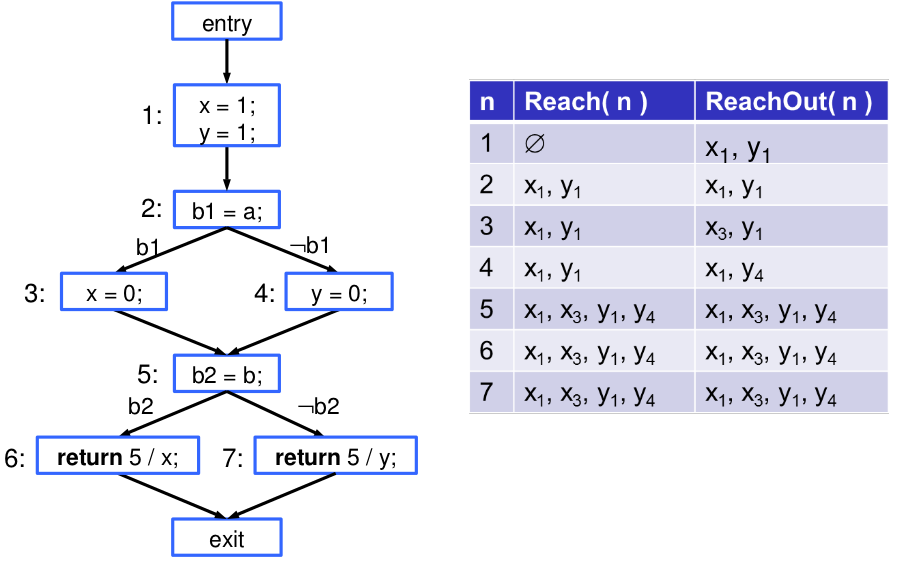
\includegraphics[width=0.5\textwidth]{img/reaching_definitions.png}
	\item DU-Pairs = $\{(d,u) | u$ \text{is a variable use for} $v$ \text{ and }$v_d \in Reach(u)\}$
\enumend

\subsection{Testing object-oriented software}

\subsubsection{Aliasing and object identities}
\enumstart
	\item Aliasing: different references that point to the same object
	\item If aliasing possible, test with aliased and non-aliased objects
\enumend

\subsubsection{Dynamically-bound method calls}
\enumstart
	\item Calls invoke different code, depending on the dynamic receivers type
	\item Testing should cover the possible behaviours
	\item A dynamically-bound call can be regarded as a case distinction on the receiver type
	\enumstart
		\item  $\rightarrow$ leads to combinatorial explosion
		\item Use semantic constraints and pairwise-combinations testing
	\enumend
\enumend

\subsubsection{Exceptions}
\enumstart
	\item Exceptions add a control flow from the block where the exception is thrown to the exit block or the block where the exception is caught
	\item Idea: cover exceptional control flow like normal control flow
	\enumstart
		\item It is impractical to represent and test all exceptional control flows
	\enumend
	\item Checked exceptions
	\enumstart
		\item Invalid conditions outside the immediate control of the program
		\item (User input, database, network, files, $\mathellipsis$)
	\enumend
	\item Unchecked exceptions
	\enumstart
		\item Defects in the program or the execution environment
		\item (Illegal arguments, null-pointer dereferences, division by zero, assertion violation, $\mathellipsis$)
	\enumend
\enumend

\subsubsection{Testing unchecked exceptions}
\enumstart
	\item Ignore unchecked exceptions thrown by other methods and virtual machine
	\item Consider throw statements
\enumend

\subsubsection{Testing checked exceptions}
\enumstart
	\item Checked exceptions represent regular control flow that needs to be tested
	\item Checked methods are declared in method signatures
	\item For each method call, add appropriate control flow edges
\enumend

\section{Program Analysis}
\enumstart
	\item Can automatically learn facts about a program
	\\ 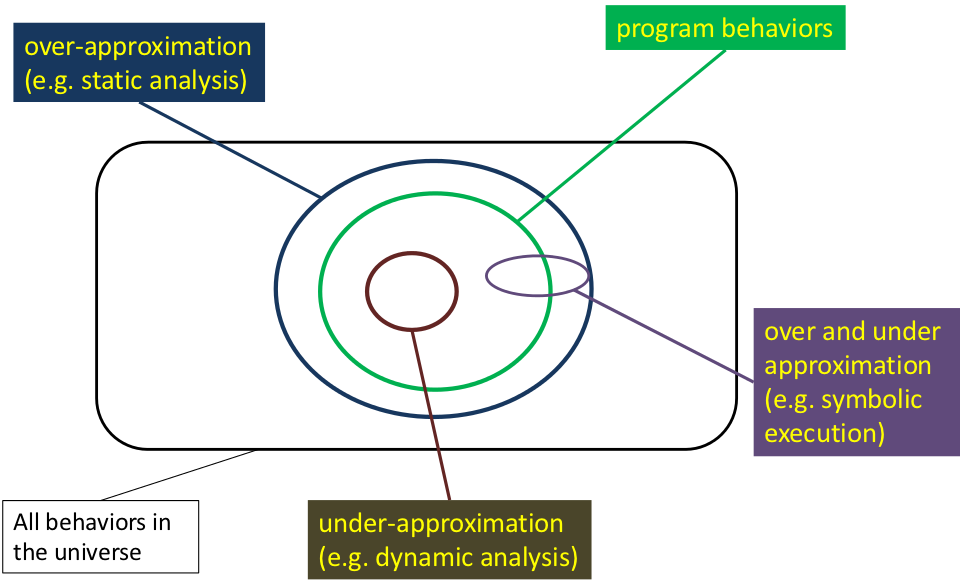
\includegraphics[width=0.5\textwidth]{img/program_analysis.png}
\enumend

\subsection{Static program analysis}
\enumstart
	\item We use abstract interpretation $\rightarrow$ a general theory of how to do approximation systematically
\enumend

\subsection{Abstract interpretation}
\enumstart
	\item Step-by-step
	\enumstart
		\item Select/define an abstract domain (depends on what you want to prove)
		\item Define abstract semantics for the language w.r.t. the domain
		\enumstart
			\item Prove sound w.r.t. concrete semantics
			\item Involves defining abstract transformers
		\enumend
		\item Iterate abstract transformers over the abstract domain $\rightarrow$ until fixpoint is reached
	\enumend
	\item The fixpoint is the over-approximation of the program
\enumend

\subsection{Abstract transformer}
\enumstart
	\item Effect of statement and expression evaluation on an abstract state
	\item Defined per programming language once and for all
	\item Abstract transformers define the abstract semantics of the language
	\item Correctness(soundness): produces a superset of what a concrete transformer would produce
	\item Precision: the set produced by the abstract transformer is as small as possible
	\item Goal, be perfectly sound and as precise as possible
	\item Sometimes, computing the most precise transformer (best transformer) is not possible
\enumend

\subsection{Iterate abstract transformers}
\enumstart
	\item Start with the least abstract element for all program-counter values
	\item Iterate the different statements/expressions and apply abstract transformers.
	\item Whenever we have two abstract elements $A$ and $B$, we can join them to produce their (least) upper bound (denoted by $A \sqcup B$)
	\item $A \sqsubseteq (A \sqcup B)$ and $B \sqsubseteq (A \sqcup B)$
	\item $D \sqsubseteq E$ means that $E$ is more abstract than $D$
	\item If it never terminates, do widening
\enumend

\subsection{Widening}
\enumstart
	\item Ensures termination at the expense of precision
	\item Do instead of join, whenever you like
\enumend

\subsection{Semantics}
\enumstart
	\item Why formal semantics?
	\enumstart
		\item Understand what a program does
		\item Implement a language
		\item Reasoning about program correctness
	\enumend
	\item Three approaches
	\enumstart
		\item Operational semantics
		\enumstart
			\item How would I execute the statement?
			\item Define a transition system, transition relation describes evaluation steps of a program
		\enumend
		\item Denotational semantics
		\enumstart
			\item What is the statement computing?
			\item Define an input/output relation that assigns meaning to each construct
		\enumend
		\item Axiomatic semantics
		\enumstart
			\item What is true after a statement is executed?
			\item Define the effect of each construct on logical statements about program store
		\enumend
	\enumend
\enumend

\subsection{SPL Language Syntax}
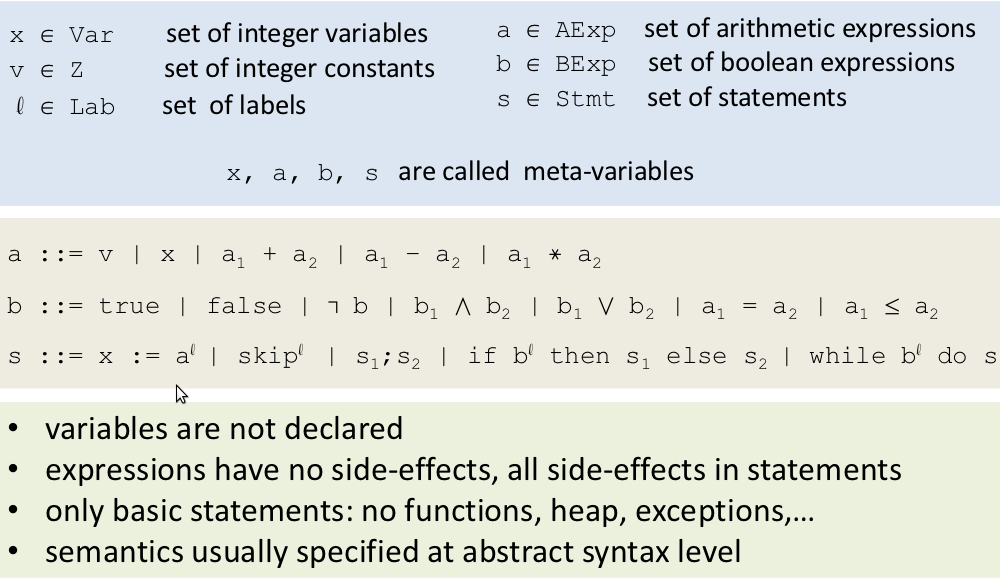
\includegraphics[width=0.5\textwidth]{img/spl_language_syntax.png}

\subsection{Operational semantics}
\enumstart
	\item Specifies how expressions and statements should be evaluated
	\item Evaluation depends on the shape of the expression/statement
	\item Evaluation depends on the values of variables
	\item Values of variables at any moment in time are given by a function $\sigma \in \text{Store} = \text{Var} \rightarrow Z$
	\item Configurations: $c \in \Sigma$ where $\Sigma = (\text{Stmt} \times \text{Store}) \cup \text{Store}$
	\enumstart
		\item $\la S, \sigma \ra$ is a configuration
		\item $\sigma$ is also a configuration, a terminal configuration
	\enumend
	\item Transitions: $\rightarrow \subseteq \Sigma \times \Sigma$ (steps between configurations)
	\item Transition system: $(\Sigma, \rightarrow, I, F)$
	\enumstart
		\item $I \subseteq \Sigma$: Initial configurations
		\item $F \subseteq \text{Store}$: final configurations
	\enumend
	\item $c \rightarrow c'$ denotes $(c, c') \in \rightarrow$
	\item $\rightarrow^*$ denotes the reflexive transitive closure of the relation $\rightarrow$
	\enumstart
		\item There is a sequence $c_0, \mathellipsis, c_n$ where $c_0 = c$, $c_n = c'$ and for all $0 \le i \le n-1$: $c_i \rightarrow c_{i+1}$
	\enumend
\enumend

\subsection{Operational semantics of SPL}

\subsubsection{Big-step semantics}
\enumstart
	\item We use it for arithmetic- and boolean expressions 
	\item $c \rightarrow c'$ describes the entire computation
	\item Some relations needed
	\enumstart
		\item $\Downarrow_a \subseteq (AExp \times Store) \times Z$
		\item $\Downarrow_b \subseteq (BExp \times Store) \times \{true, false\}$
		\item $\la a, \sigma \ra \Downarrow_a v$ means: "expression $a$ evaluates to $v$ in store $\sigma$"
	\enumend
	\item Evaluation rules for arithmetic expressions
	\enumstart
		\item $\frac{\la a_1, \sigma \ra \Downarrow_a v_1 \ \ \ \la a_2, \sigma \ra \Downarrow_a v_2}{\la a_1 + a_2, \sigma \ra \Downarrow_a v_1 + v_2}$
		\item $\frac{}{\la x, \sigma \ra \Downarrow_a \sigma(x)}$
	\enumend
	\item Evaluation rules for boolean expressions
	\enumstart
		\item $\frac{\la a_1, \sigma \ra \Downarrow_a v_1 \ \ \ \la a_2, \sigma \ra \Downarrow_a v_2}{\la a_1 \le a_2, \sigma \ra \Downarrow_b bv}$ bv is $v_1 \le v_2$
		\item $\frac{\la a_1, \sigma \ra \Downarrow_a v_1 \ \ \ \la a_2, \sigma \ra \Downarrow_a v_2}{\la a_1 = a_2, \sigma \ra \Downarrow_b bv}$ bv is $v_1 == v_2$
		\item $\frac{\la b_1, \sigma \ra \Downarrow_b true \ \ \ \la b_2, \sigma \ra \Downarrow_b true}{\la b_1 \land b_2, \sigma \ra \Downarrow_b true}$
		\item $\frac{\la b_1, \sigma \ra \Downarrow_b false}{\la b_1 \land b_2, \sigma \ra \Downarrow_b false}$
		\item $\frac{\la b_2, \sigma \ra \Downarrow_b false}{\la b_1 \land b_2, \sigma \ra \Downarrow_b false}$ adsf
	\enumend
\enumend

\subsubsection{Small-step semantics}
\enumstart
	\item We use it for statements
	\item $c \rightarrow c'$ describes a single step of a larger computation
	\item Evaluating a statement produces a new store ($\la s, \sigma \ra \rightarrow \la s', \sigma' \ra$)
	\item Evaluation order is important
	\enumstart
		\item In "$s_1;s_2$", $s_1$ is evaluated before $s_2$
		\item In "if true then $s_1$ else $s_2$", $s_2$ is not evaluated
	\enumend
	\item Evaluation rules for Stmt
	\enumstart
		\item $\frac{\la s_1, \sigma \ra \rightarrow \la s_2, \sigma_1 \ra}{\la s_1;s_3, \sigma \ra \rightarrow \la s_2;s_3, \sigma_1 \ra}$ bla
		\item $\frac{\la s_1, \sigma \ra \rightarrow \sigma_1}{\la s_1;s_2, \sigma \ra \rightarrow \la s_2, \sigma_1 \ra}$
		\item $\frac{}{\la skip, \sigma \ra \rightarrow \sigma}$
		\item $\frac{\la a, \sigma \ra \Downarrow_a v}{\la x := a, \sigma \ra \rightarrow \la x := v, \sigma \ra}$
		\item $\frac{}{\la x := v, \sigma \ra \rightarrow \sigma[x \mapsto v]}$
		\item $\frac{}{\la \text{if true then } s_1 \text{ else } s_2, \sigma \ra \rightarrow \la s_1, \sigma \ra}$
		\item $\frac{}{\la \text{if false then } s_1 \text{ else } s_2, \sigma \ra \rightarrow \la s_2, \sigma \ra}$
		\item $\frac{\la b_1, \sigma \ra \Downarrow_b bv}{\la \text{if } b_1 \text{ then } s_1 \text{ else } s_2, \sigma \ra \rightarrow \la \text{if } bv \text{ then } s_1 \text{ else } s_2, \sigma \ra}$
		\item $\frac{}{\la \text{while } b \text{ do } s, \sigma \ra \rightarrow \la \text{if } b \text{ then } (s; \text{while } b \text{ do } s) \text{ else } skip, \sigma}$
		\item blub
	\enumend
	\item Sequences
	\enumstart
		\item For a program $s_0$ the steps are formed via the relation $\rightarrow$.
		\item $\Downarrow_a$ and $\Downarrow_b$ are only used to justify the steps with $\rightarrow$
		\item $\Downarrow_a$ and $\Downarrow_b$ are only used to build the relation $\rightarrow$
	\enumend
\enumend

\subsection{Trace semantics}
\enumstart
	\item Trace semantics are the set of all program traces starting from initial configurations
	\item $\llbracket P \rrbracket = \{c_0, \mathellipsis, c_{n - 1} \ | \ n \ge 1 \land c_0 \in I \land \forall i \in [0, n - 2]: c_i \rightarrow c_{i + 1}\}$
	\item Traces need not end in final configurations
	\item Traces are of finite length, but the number of initial configurations can be infinite
	\item Overapproximate a function
	\enumstart
		\item Consider a function $F$
		\item $F(\llbracket P \rrbracket) = \llbracket P \rrbracket \implies \llbracket P \rrbracket $ is a fixed point of $F$
		\item Discover a function $F^\#$ such that $F^\#$ approximates $F$
		\item A fixed point of $F^\#$ approximates a fixed point of $F$
		\item Compute a fixed point of $F^\# \implies F^\#(\llbracket P \rrbracket^\#) = \llbracket P \rrbracket^\#$
	\enumend
\enumend

\subsection{Mathematical Background}

\subsubsection{Structures}
\enumstart
	\item They define the concrete and abstract domain
\enumend

\paragraph{Partially ordered sets (posets)}
\enumstart
	\item A partial order is a relation $\sqsubseteq \ \subseteq L \times L$ on a set $L$
	\item The following properties hold
	\enumstart
		\item Reflexive: $\forall p \in L: p \sqsubseteq p$
		\item Transitive: $\forall p,q,r \in L: p \sqsubseteq q \land q \sqsubseteq r \implies p \sqsubseteq r$
		\item Anti-symmetric: $\forall p,q \in L: p \sqsubseteq q \land q \sqsubseteq p \implies p = q$
	\enumend
	\item A poset $(L, \sqsubseteq)$ is a set $L$ equipped with a partial ordering $\sqsubseteq$
	\item $\bot \in L$ is called the least element if it is smaller than all other elements of the poset. $\forall p \in L: \bot \sqsubseteq p$
	\item $\top \in L$ is called the greatest element if it is greater than all other elements of the poset. $\forall p \in L: p \sqsubseteq \top$
	\item The least and greatest elements may not exist, but if they do they are unique
	\item Given $(L, \sqsubseteq)$ and $Y \subseteq L$
	\enumstart
		\item $u \in L$ is an upper bound of $Y$ if $\forall p \in Y: p \sqsubseteq u$
		\item $v \in L$ is a lower bound of $Y$ if $\forall p \in Y: v \sqsubseteq p$
		\item $\sqcup Y \in L$ is a least upper bound of $Y$ if
		\enumstart
			\item $\sqcup Y$ is an upper bound of $Y$ and
			\item $\forall u: u =$ upperBound($Y$) $\implies \sqcup Y \sqsubseteq u$
		\enumend
		\item $\sqcap Y \in L$ is a greatest lower bound of $Y$ if
		\enumstart
			\item $\sqcap Y$ is a lower bound of $Y$ and
			\item $\forall u: u =$ lowerBound($Y$) $\implies u \sqsubseteq \sqcap Y$
		\enumend
		\item Bounds may not exist and may not be in $Y$
		\item We write $p \sqcup q$ for $\sqcup\{p, q\}$ and $p \sqcap q$ for $\sqcap\{p, q\}$
	\enumend
\enumend

\paragraph{Complete lattices}
\enumstart
	\item A complete lattice $(L, \sqsubseteq, \sqcup)$ is a poset, where $\sqcup Y$ and $\sqcap Y$ exist for any $Y \subseteq L$
	\item The set of traces $\llbracket P \rrbracket$ belongs to a complete lattice
\enumend

\paragraph{Chains}
\enumstart
	\item Given a poset $(L, \sqsubseteq)$, a subset $Y \subseteq L$ is a chain if every two elements in $Y$ are comparable. $\forall x,y \in Y: (x \sqsubseteq y) \lor (y \sqsubseteq x)$
	\item The height of the poset is the chain with the largest size
\enumend

\subsubsection{Functions}
\enumstart
	\item A function $f: A \rightarrow B$ between two posets $(A, \sqsubseteq)$ and $(B, \le)$ is monotone if: $\forall a,b \in A: a \sqsubseteq b \implies f(a) \le f(b)$
	\item For a poset $(L, \sqsubseteq)$, a function $f: L \rightarrow L$ and an element $x \in L$:
	\enumstart
		\item $x$ is a fixed point iff $f(x) = x$
		\item $x$ is a post-fixed point iff $f(x) \sqsubseteq x$
		\item Fix($f$) denotes the set of all fixed points
		\item Red($f$) denotes the set of all post-fixed points
		\item lfp$^\sqsubseteq f \in L$ is a least fixed point of $f$ iff:
		\enumstart
			\item lfp$^\sqsubseteq f$ is a fixed point
			\item $\forall a \in L: a = f(a) \implies$ lfp$^\sqsubseteq f \sqsubseteq a$
			\item The least fixed point may not exist
		\enumend
	\enumend
	\item Tarski's fixed point theorem: if $(L,\sqsubseteq, \sqcup, \sqcap, \bot, \top)$ is a complete lattice anf $f: L \rightarrow L$ is monotone:
	\enumstart
		\item lfp$^\sqsubseteq f$ exists, and
		\item lfp$^\sqsubseteq f = \sqcap$Red($f$)$\in$ Fix($f$) 
	\enumend
	\item Computation of fixed points
	\enumstart
		\item For a poset $(L, \sqsubseteq)$, a function $f: L \rightarrow L$, an element $a \in L$ the iterates of the function from $a$ are
		\enumstart
			\item $f^0(a), f^1(a), f^2(a), \mathellipsis$
			\item $f^{n+1}(a) = f(f^n(a))$
			\item $f^0(a) = a$
		\enumend
		\item Given a poset of finite height, a least element $\bot$ and a monotone $f$
		 \enumstart
		 	\item $f^0(\bot), f^1(\bot), f^2(\bot), \mathellipsis$ form an increasing sequence
		 	\item $\exists n \in \N: f^n(\bot) = f^{n+1}(\bot)$
		 	\item lfp$^\sqsubseteq f = f^n(\bot)$
		 \enumend
		 \item $\PTrace$ is the least fixed point of $F(S) = I \cup \{\pi \cdotp c \cdotp c' \ | \ \pi \cdotp c \in S \land c \rightarrow c'\}$
		 \item The set of traces $\PTrace$ is an element of a complete lattice
	\enumend
\enumend

\subsubsection{Gallois connections}
\enumstart
	\item Left $(L_1, \sqsubseteq_1, \sqcup_1, \sqcap_1)$ and $(L_2, \sqsubseteq_2, \sqcup_2, \sqcap_2)$ be complete lattices and let $\alpha: L_1 \rightarrow L_2$ and $\gamma: L_2 \rightarrow L_1$. Then $\alpha$ and $\gamma$ form a gallois connection if
	\enumstart
		\item $\alpha$ is monotone
		\item $\gamma$ is monotone
		\item $\alpha \circ \gamma$ is reductive: $\forall x_2 \in L_2: \alpha(\gamma(x_2)) \sqsubseteq_2 x_2$
		\item $\gamma \circ \alpha$ is extensive: $\forall x_1 \in L_1: x_1 \sqsubseteq_1 \gamma(\alpha(x_1))$
	\enumend
	\item Intuition
	\enumstart
		\item $\alpha$ and $\gamma$ monotone $\rightarrow$ relationship between information in the concrete is preserved in the abstract and vice versa
		\item $\gamma \circ \alpha$ extensive $\rightarrow \alpha$ is a correct approximation 
		\item $(L_1, \sqsubseteq_1, \sqcup_1, \sqcap_1) \Gallois[] (L_2, \sqsubseteq_2, \sqcup_2, \sqcap_2)$
		\enumstart
			\item The concrete is captured by the lattice on the left
			\item The abstract is captured by the lattice on the right
			\item $\alpha$ is the abstraction function
			\item $\gamma$ is the concretization function
			\item Concrete and abstract are linked by this connection
		\enumend
	\enumend
	\item Another definition
	\enumstart
		\item $\forall x_1 \in L_1, \forall x_2 \in L_2: \alpha(x_1) \sqsubseteq_2 x_2 \Leftrightarrow x_1 \sqsubseteq_1 \gamma(x_2)$
	\enumend
	\item $\alpha$ uniquely determines $\gamma$ and vice versa
	\enumstart
		\item $\alpha(x) = \sqcap_2\{z \ | \ x \sqsubseteq_1 \gamma(z)\}$
		\item $\gamma(z) = \sqcup_1\{x \ | \ \alpha(x) \sqsubseteq_2 z\}$
	\enumend
	\item Composition
	\enumstart
		\item Given: $(L_1, \sqsubseteq_1, \sqcup_1, \sqcap_1) \Gallois[1] (L_2, \sqsubseteq_2, \sqcup_2, \sqcap_2)$
		\item Given: $(L_2, \sqsubseteq_2, \sqcup_2, \sqcap_2) \Gallois[2] (L_3, \sqsubseteq_3, \sqcup_3, \sqcap_3)$
		\item $\implies (L_1, \sqsubseteq_1, \sqcup_1, \sqcap_1) \leftrightarrows^{\gamma_1 \circ \gamma_2}_{\alpha_1 \circ \alpha_2} (L_3, \sqsubseteq_3, \sqcup_3, \sqcap_3)$ 
	\enumend
\enumend

\subsubsection{Function Approximation}
\enumstart
	\item We want to compute an over-approximation of the least fixed point of a function
	\item We want to avoid computing the least fixed point of a function (might not be feasible)
	\item Given: $f: A \rightarrow B$, $g: A \rightarrow B$
	\enumstart
		\item $g$ approximates $f$ iff $\forall x \in A: f(x) \le g(x)$
	\enumend
	\item Given: $(L_1, \sqsubseteq_1, \sqcup_1, \sqcap_1) \Gallois (L_2, \sqsubseteq_2, \sqcup_2, \sqcap_2)$, $f: L_1 \rightarrow L_1$ and $g: L_2 \rightarrow L_2$
	\enumstart
		\item $g$ approximates $f$ iff $\forall x \in L_1, \forall z \in L_2: \alpha(x) \sqsubseteq_2 z \implies \alpha(f(x)) \sqsubseteq_2 g(z)$
		\item When $f$ and $g$ are monotone: $\forall z \in L_2: \alpha(f(\gamma(z))) \sqsubseteq_2 g(z)$
	\enumend
	\item Least precise approximation $g(z) = \top$ (not very usefull)
	\item Most precise approximation $g(z) = \alpha(f(\gamma(z)))$ (best abstract function,  best transformer)
	\item $\alpha($lfp$(f)) \sqsubseteq_2 $ lfp$(g)$
\enumend

\subsection{Formal concepts illustrated}
\enumstart
	\item Domain of traces $(\mathcal{P}(\Sigma^+), \subseteq, \cup, \cap, \emptyset, \Sigma^+)$ is a complete lattice, where
	\enumstart
		\item $\Sigma =$ Lab $\times$ Store
		\item $\Sigma^+$ denotes all finite traces
	\enumend
	\item Traces in $\Sigma^+$ that belong to $\PTrace$
	\\ 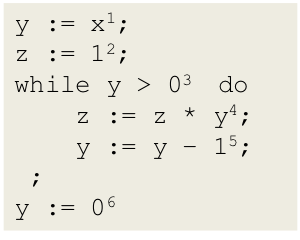
\includegraphics[width=0.2\textwidth]{img/sample_program.png}
	\enumstart
		\item e.g. $\langle 1, \{x \mapsto 42, y \mapsto 0, z \mapsto 0\} \rangle \cdotp \langle 2, \{x \mapsto 42, y \mapsto 42, z \mapsto 0\} \rangle \cdotp \langle 3, \{x \mapsto 42, y \mapsto 42, z \mapsto 1\} \rangle \cdotp \mathellipsis$
		\item "$\cdotp$" denotes concatenation
		\item A trace is just a sequence of states, need not follow the program transition relation $\rightarrow$
	\enumend
	\item Abstraction
	\enumstart
		\item $\PTrace$ can be infinite $\rightarrow$ create abstraction
		\item State abstraction $\rightarrow$ $(\mathcal{P}(\Sigma), \subseteq, \cup, \cap, \emptyset, \Sigma)$ forms a complete lattice
		\enumstart
			\item $\alpha^s:  \mathcal{P}(\Sigma^+) \rightarrow \mathcal{P}(\Sigma)$, $\alpha^s(Traces) = \{\pi_i \ | \ i \in [0, |\pi|] \land \pi \in Traces\}$
			\item We lose the relationship between states
			\item We lose how many times each state occurs in a trace
			\item $\gamma^s: \mathcal{P}(\Sigma) \rightarrow \mathcal{P}(\Sigma^+)$, $\gamma^s(S) = \{c_0 \cdotp \mathellipsis, c_n \ | \ n \ge 0 \land \forall i \in [0, n]: c_i \in S\}$
			\item Or by general formula: $\gamma^s(S) = \cup \{traces \subseteq \Sigma^+ \ | \ \alpha^s(traces) \subseteq S\}$
			\item This forms a gallois connection
		\enumend
		\item Invariance abstraction
		\enumstart
			\item $\Sigma =$ Lab $\times$ Store
			\item $\alpha^{inv}: \mathcal{P}($Lab $\times$ Store$) \rightarrow ($Lab $\rightarrow \mathcal{P}($Store$)): \alpha^{inv}(S)\ell = \{\sigma \ | \ \langle \ell, \sigma \rangle \in S\}$
			\item Abstract domain: $($Lab$ \rightarrow \mathcal{P}($Store$), \dot \subseteq, \dot \cup, \dot \cap, \lambda \ell.\emptyset, \lambda \ell.$Store$)$
			\item $f \dot \subseteq g$ means that for any value $x \in X: f(x) \subseteq g(x)$
			\item $f \dot \cup g$ produces a new function $\lambda x \in X. f(x) \cup g(x)$
			\item Does not lose information
			\item $\gamma^{inv}: ($Lab $\rightarrow \mathcal{P}($Store$)) \rightarrow \mathcal{P}($Lab $\times$ Store$): \gamma^{inv}(M) = \{\langle \ell, \sigma \rangle \ | \ \sigma \in M(\ell)\}$
			\item This forms a gallois connection
		\enumend
		\item Cartesian abstraction
		\enumstart
			\item Abstraction that loses relationship between variables
			\item $\alpha^x: ($Lab$ \rightarrow \mathcal{P}($Store$)) \rightarrow ($Lab$ \rightarrow ($Var$ \rightarrow \Z)): \alpha^x(F)(\ell)x = \{\sigma(x) \ | \ \sigma \in F(\ell)\}$
			\item $\gamma^x(M)\ell = \cup \{$stores $\subseteq \Sigma \ | \ \alpha^x(\ell \rightarrow $ stores$) \subseteq \ell \rightarrow M(\ell)\}$
			\item This forms a gallois connection
		\enumend
		\item Interval abstraction
		\enumstart
			\item Interval domain: $(L^i, \sqsubseteq_i, \sqcup_i, \sqcap_i, \bot_i, [-\infty, \infty])$
			\item $\Z^\infty = \Z \cup \{-\infty, \infty\}$
			\item $L^i = \{[x,y] \ | \ x,y \in \Z^\infty, x \le y\} \cup \bot_i$
			\item For $S \subseteq \Z^\infty$
			\enumstart
				\item min(S) = minimum number in $S$
				\item max(S) = maximum number in $S$
			\enumend
			\item $[a,b] \sqsubseteq_i [c,d]$ if $a \ge c \land b \le d$
			\item $[a,b] \sqcup_i [c,d] = [$min$(\{a,c\}), $max$(\{b,d\})]$
			\item $[a,b] \sqcap_i [c,d] = $meet$($max$(\{a,c\}),$min$(\{b,d\}))$
			\item where meet$(a,b) = [a,b]$ if $a \le b$ and $\bot$ otherwise
			\item $\alpha^i: ($Lab $ \rightarrow ($Var $ \rightarrow \mathcal{P}(\Z))) \rightarrow ($Lab $\rightarrow ($Var $\rightarrow L^i))$
			\item $\alpha^i(C)(\ell)x = [$min$(C(\ell)x), $max$(C(\ell)x)]$ if $C(\ell)x \ne \emptyset$ and $\bot_i$ otherwise
			\item $\gamma^i(M)(\ell)x = \{v \in \Z \ | \ l \le v \land  v \le u\}$ if $M(\ell)x = [l, u]$ and $\emptyset$ otherwise
		\enumend
		\item chaining the abstractions
		\enumstart
			\item $\alpha^i \circ \alpha^x \circ \alpha^{inv} \circ \alpha^s(\PTrace)$
			\item $F^i$ is the best transformer of $F$
			\item $F^i = \alpha^i \circ \alpha^x \circ \alpha^{inv} \circ \alpha^s \circ F \circ \gamma^s \circ \gamma^{inv} \circ \gamma^x \circ \gamma^i$
		\enumend
	\enumend
\enumend

\subsection{Definitions}
\enumstart
	\item $(\ell, action, \ell')$ is an edge in the control-flow graph
	\item if $t = \langle \ell, \sigma \rangle \rightarrow \langle \ell', \sigma' \rangle$ exists in $\PTrace$ where $t$ was performed by $action: (\ell, action, \ell')$ exists
	\item an $action$ can be:
	\enumstart
		\item $b \in$ BExp
		\item $x := a$
		\item skip
	\enumend
	\item $\llbracket action \rrbracket_i$ is an abstract transformer
	\enumstart
		\item if the map contains a variable mapped to $\bot_i$ then the result of the transformer is $\bot$
		\item otherwise apply the rules
	\enumend
	\item $\llbracket x := a\rrbracket_i(m) = m[x \mapsto v]$, where $\langle a,m \rangle \Downarrow_i v$
	\item Arithmetic expressions
	\enumstart
		\item Addition $\llbracket \rrbracket$
		\enumstart
			\item if we add $\bot_i$ to anything, we get $\bot_i$
			\item otherwise $[a,b]+[c,d] = [a+c, b+d]$
		\enumend
	\enumend
	\item Conditionals $\llbracket a_1 \ c \ a_2 \rrbracket_i$
	\enumstart
		\item $c \in \{\le, =, < \}$
		\item $\llbracket a_1 \ c \ a_2 \rrbracket_i(m) = $select$(a_1, r_1, m) \sqcap $select$(a_2, r_2, m)$, $(r_1, r_2) = pair_c(\langle a_1, m \rangle \Downarrow_i, \langle a_2, m \rangle \Downarrow_i)$
		\item When $a$ is a constant
		\enumstart
			\item select$(a,r,m) = m$ if $a \sqcap_i r \ne \bot_i$ and $\bot$ otherwise		\enumend
		\item When $a$ is a variable
		\enumstart
			\item select$(a,r,m) = m[a \mapsto (r \sqcap_i m(a))]$
		\enumend
		\item $pair_\le([l_1, u_1], [l_2, u_2]) = ([l_1, u_1] \sqcap_i [-\infty, u_2], [l_1, \infty] \sqcap_i [l_2, u_2])$
	\enumend
	\item Boolean expressions $\llbracket b\rrbracket_i$
	\enumstart
		\item $\llbracket b_1 \lor b_2 \rrbracket_i(m) = \llbracket b_1 \rrbracket_i(m) \sqcup_i \llbracket b_2\rrbracket_i(m)$
		\item $\llbracket b_1 \land b_2 \rrbracket_i(m) = \llbracket b_1 \rrbracket_i(m) \sqcap_i \llbracket b_2\rrbracket_i(m)$
	\enumend
	\item The widening operator $\widen$
	\enumstart
		\item $\widen: L \times L \rightarrow L$
		\item $\forall a, b \in L: (a \sqcup b) \sqsubseteq (a \widen b)$ (approximates the join)
		\item If $L$ is a complete lattice, $F: L \rightarrow L$ is monotone, then
		\item $y^0 = \bot, y^n = y^{n-1} \widen F(y^{n-1})$ will stabilize after a finite number of steps with $y^n$ beeing a post-fixed point of F
	\enumend
	\item Widening for intervals
	\enumstart
		\item $\widen_i: L^i \times L^i \rightarrow L^i$
		\item if one of the operands is $\bot$, the result is the other operand
		\item $[a,b] \widen_i [c,d] = [e,f]$, where
		\enumstart
			\item if $c < a$ then $e = -\infty$ else $e = a$
			\item if $d > b$ then $f = \infty$ else $f = b$
		\enumend
	\enumend
\enumend

\subsection{Relational domains}
\enumstart
	\item Relational domains keep the relation between variables
\enumend

\subsubsection{Octagon domain}
\enumstart
	\item Constraints are of the form $\pm x \pm y \le(\ge) c$
	\item The slope is fixed $\rightarrow$ octagon shape
	\item A more spezialized polyhedra domain
	\item More efficient in space and time than polyhedra domain
\enumend

\subsubsection{Polyhedra domain}
\enumstart
	\item Constraints are of the form $c_1x_1 + c_2x_2 + \mathellipsis + c_nx_n \le(\ge) c$
	\item The slope can vary
	\item More precise than octogon domain
\enumend

\subsection{Predicate abstraction}
\enumstart
	\item Is a particular instance of abstract interpretation
	\item Step-by-step
	\enumstart
		\item Concrete domain
		\enumstart
			\item Start with: Lab $\rightarrow \mathcal{P}($Store$)$
			\item Then go to: Lab $\rightarrow$ FOL (first-order logic formula) by gallois connection
		\enumend
		\item Concrete transformers (weakest pre-/stronges post-condition
		\enumstart
			\item We have a function $F^{fol}: ($Lab $\rightarrow$ FOL$) \rightarrow ($Lab $\rightarrow$ FOL$)$ which overapproximates the function $F$
			\item $F^{fol}(m)\ell = true$ if $\ell$ is initial label and $\lor_{(\ell', action, \ell)} \llbracket action \rrbracket_{fol}(m(\ell'))$ otherwise
			\item The best transformer for $\llbracket action \rrbracket_{fol}:$ FOL $\rightarrow$ FOL is the strongest postcondition $sp$
			\item $\llbracket action \rrbracket_{fol} \varphi = sp(\varphi, $action$)$
			\item $sp(\varphi,$ action$) = \psi$
			\item $sp(\varphi, x := a) = \exists v: x = a[v/x] \land \varphi[v/x]$
			\item FOL is semi-decidable $\rightarrow$ We can't guarantee termination
			\item Weakest pre- vs. strongest postcondition: $sp(\varphi,$ action$) \implies \psi$ iff $\varphi \implies wp(\psi, $action$)$
		\enumend
		\item Abstract domain
		\enumstart
			\item Built from a finite set of predicates $F = \{\varphi_1, \mathellipsis, \varphi_n\}$
			\item We assume that there are no two formulas in $F$ that are equivalent
			\item Each element of the abstract domain is called a cube
			\item A cube is a formula, which is a conjunction of some elements of $F$ or their negations
			\item Each $\varphi_i$ is allowed to appear at most once
			\item $false$ is also considered a cube (and $true$ as it's negation)
			\item The abstract domain is: Lab $\rightarrow$ Cube$_F$
			\item $(a \sqsubseteq_{pa} b) = (a \implies b)$
			\item $(a \sqcup_{pa} b)$ is a predicate that contains all cubes that appear in $a$ and in $b$
			\item If all predicates are omitted: return $true$
			\item $(a \sqcap_{pa} b)$: keep all predicates $\varphi_k$ of $a$ if $b$ doesn't contain it's negation and vice-versa
			\item If $a$ and $b$ contradict each other: return $false$
		\enumend
		\item Galois connection
		\enumstart
			\item $\gamma($cube$) = c$ where cube $\Leftrightarrow$ c
			\item $\alpha(\psi) = \and^n_{i=1}\{c_i \ | \ \psi \implies c_i\}$
		\enumend
		\item Transformers in the abstract domain
		\enumstart
			\item $\llbracket $action$ \rrbracket_{pa}($cube$) = \land \{c_i \ | \ $cube $\implies wp(c_i,$ action$)\}$
			\item The validity of cube $\implies wp(c_i,$ action$)$ is usually thecked with an SMT solver
		\enumend
		\item Fixed point computation
	\enumend
\enumend


\end{document}